\section{Ergebnisse des Fragebogens}
\label{sec:anhang-fragebogen}

Im Folgenden werden die Fragen und Antworten des Online Fragebogens ausführlich dargestellt. Die Anzahl der Teilnehmer kann dabei variieren, da manche Fragen als Pflichtfragen deklariert wurden und andere nicht. Ob die Frage eine Pflichtfrage ist, Single- oder Multiple-Choice und wie viele der Teilnehmer die Frage beantwortet haben, ist jeweils nachstehend kurz angegeben.

\begin{enumerate}
    \item \textbf{Wie häufig buchst du einen Raum?} \\
    Pflichtfrage, Single-Choice, Anzahl Teilnehmer: 46
    \begin{itemize}
        \item[] 6 (13,0\,\%): täglich
        \item[] 14 (30,4\,\%): alle 2-3 Tage
        \item[] 10 (21,7\,\%): wöchentlich
        \item[] 9 (19,6\,\%): monatlich
        \item[] 7 (15,2\,\%): nie
    \end{itemize}
    
    \item \textbf{Wie lange im Voraus buchst du in der Regel einen Raum?} \\ 
    Pflichtfrage, Single-Choice, Anzahl Teilnehmer: 46
    \begin{itemize}
        \item[] 4 (8,7\,\%): unmittelbar
        \item[] 4 (8,7\,\%): am selben Tag
        \item[] 11 (23,9\,\%): ein Tag
        \item[] 17 (37,0\,\%): mehrere Tage
        \item[] 1 (2,2\,\%): Wochen/Monate
        \item[] 9 (19,6\,\%): Ich habe noch nie einen Raum gebucht
    \end{itemize}
    
    \item \textbf{Wie lange dauern deine Besprechungen in der Regel?} \\ 
    Keine Pflichtfrage, Single-Choice, Anzahl Teilnehmer: 46
    \begin{itemize}
        \item[] 13 (28,3\,\%): < 1 Std.
        \item[] 30 (65,2\,\%): 1 - 2 Std.
        \item[] 3 (6,5\,\%): 2 - 3 Std.
        \item[] 0 (0,0\,\%): 3 - 4 Std.
        \item[] 0 (0,0\,\%): > 4 Std.
    \end{itemize}
    
    \item \textbf{Wie oft stimmt die gebuchte Dauer eines Termins mit der tatsächlichen überein?} 
    \\ 
    Keine Pflichtfrage, Single-Choice, Anzahl Teilnehmer: 38
    \begin{itemize}
        \item[] 9 (23,7\,\%): sehr oft
        \item[] 21 (55,3\,\%): oft
        \item[] 3 (7,9\,\%): ausgeglichen
        \item[] 5 (13,2\,\%): selten
        \item[] 0 (0,0\,\%): sehr selten
    \end{itemize}
    
    \item \textbf{Wie oft wird ein Meeting beendet, weil die Buchung des Raums abgelaufen ist, obwohl noch Gesprächsbedarf bestehen würde?} \\ 
    Keine Pflichtfrage, Single-Choice, Anzahl Teilnehmer: 38
    \begin{itemize}
        \item[] 1 (2,6\,\%): sehr oft
        \item[] 7 (18,4\,\%): oft
        \item[] 10 (26,3\,\%): ausgeglichen
        \item[] 15 (39,5\,\%): selten
        \item[] 5 (13,2\,\%): sehr selten
    \end{itemize}
    
    \item \textbf{Hast du beim Buchen von Räumen einen festen oder flexiblen Zeitpunkt?} \\ 
    Keine Pflichtfrage, Single-Choice, Anzahl Teilnehmer: 44
    \begin{itemize}
        \item[] 4 (9,1\,\%): fest
        \item[] 8 (18,2\,\%): eher fest
        \item[] 19 (43,2\,\%): ausgeglichen
        \item[] 7 (15,9\,\%): eher flexibel
        \item[] 6 (13,6\,\%): flexibel
    \end{itemize}
    
    \item \textbf{Wie oft benutzt du den Slackbot Joan?} \\ 
    Pflichtfrage, Single-Choice, Anzahl Teilnehmer: 46
    \begin{itemize}
        \item[] 1 (2,2\,\%): jede Buchung
        \item[] 2 (4,3\,\%): eher fest
        \item[] 2 (4,3\,\%): ausgeglichen
        \item[] 0 (0,0\,\%): Selten
        \item[] 41 (89,1\,\%): nie
    \end{itemize}
    
    \item \textbf{Nutzt du das E-Paper Display an den Räumen, wenn du sofort einen Raum benötigst?} \\ 
    Pflichtfrage, Single-Choice, Anzahl Teilnehmer: 46
    \begin{itemize}
        \item[] 16 (34,8\,\%): immer
        \item[] 15 (32,6\,\%): oft
        \item[] 5 (10,9\,\%): ausgeglichen
        \item[] 5 (10,9\,\%): selten
        \item[] 5 (10,9\,\%): nie
    \end{itemize}
    
    \item \textbf{Nutzt du das E-Paper Display an den Räumen, wenn zu einem späteren Zeitpunkt den Raum verwenden möchtest} \\ 
    Pflichtfrage, Single-Choice, Anzahl Teilnehmer: 46
    \begin{itemize}
        \item[] 1 (2,2\,\%): immer
        \item[] 3 (6,5\,\%): oft
        \item[] 5 (10,9\,\%): ausgeglichen
        \item[] 9 (19,6\,\%): selten
        \item[] 28 (60,9\,\%): nie
    \end{itemize}
    
    \item \textbf{Wie oft stimmt deiner Erfahrung nach der Belegungsstatus des Raumes mit den Angaben auf dem E-Paper Display überein?} \\ 
    Pflichtfrage, Single-Choice, Anzahl Teilnehmer: 46
    \begin{itemize}
        \item[] 3 (6,5\,\%): immer
        \item[] 11 (23,9\,\%): oft
        \item[] 21 (45,7\,\%): ausgeglichen
        \item[] 11 (23,9\,\%): selten
        \item[] 0 (0,0\,\%): nie
    \end{itemize}
    
    \item \textbf{Wie oft benötigst du bei deinen Meetings bestimmtes Equipment?} \\
    Gemeint ist damit Equipment, das nicht standardmäßig in den Räumen vorhanden ist, also etwas anderes als AppleTV, Fernseher, Whiteboard. \\ 
    Pflichtfrage, Single-Choice, Anzahl Teilnehmer: 46
    \begin{itemize}
        \item[] 1 (2,2\,\%): immer
        \item[] 19 (41,3\,\%): oft
        \item[] 5 (10,9\,\%): ausgeglichen
        \item[] 15 (32,6\,\%): selten
        \item[] 6 (13,0\,\%): nie
    \end{itemize}
    
     \item \textbf{Wie führst du deine Raumbuchungen aktuell am häufigsten durch?} \\ 
     Pflichtfrage, Single-Choice, Anzahl Teilnehmer: 46
    \begin{itemize}
        \item[] 39 (84,8\,\%): Computer - Web Interface
        \item[] 7 (15,2\,\%): Ich habe noch nie einen Raum gebucht
        \item[] 0 (0,0\,\%): Smartphone - Web Interface
        \item[] 0 (0,0\,\%): Slackbot Joan
    \end{itemize}
    
    \item \textbf{Wie würdest du deine Raumbuchung am liebsten durchführen?} \\ 
    Pflichtfrage, Single-Choice, Anzahl Teilnehmer: 46
    \begin{itemize}
        \item[] 34 (73,9\,\%): Computer - Web Interface
        \item[] 5 (10,9\,\%): Smartphone - Applikation
        \item[] 3 (6,5\,\%): Computer - Anwendung
        \item[] 3 (6,5\,\%): Slackbot Joan
        \item[] 1 (2,2\,\%): Smartphone - Web Interface
    \end{itemize}
    
    \item \textbf{Wie fändest du es, wenn du die Raumbuchung bestätigen müsstest?} \\ 
    Pflichtfrage, Single-Choice, Anzahl Teilnehmer: 46
    \begin{itemize}
        \item[] 11 (23,9\,\%): gut
        \item[] 15 (32,6\,\%): eher gut
        \item[] 6 (13,0\,\%): neutral
        \item[] 6 (13,0\,\%): eher schlecht
        \item[] 8 (17,4\,\%): schlecht
    \end{itemize}
    
    Begründungen:
    \begin{itemize}
        \item ich nicht weiß ob immer daran denke [Auswahl: neutral]
        \item ich sicherlich nicht daran denke, denn nach der Raumbuchung (die nicht abgelehnt wird) ist die Sache bei mir abgehakt [Auswahl: schlecht]
        \item Dann Räume auch wieder frei werden, allerdings sollte das Zeitintervall schon auch ein paar Minuten -> 15/20 tolerieren [Auswahl: eher gut]
        \item der Raum bei nicht Benutzung als frei markiert ist somit weiter verwendbar [Auswahl: eher gut]
        \item weil dann sicher ist welches Meeting in dem Raum ist, falls man zb zu spät kommt, wissen will das genau das meeting um zb 13 Uhr zu ende ist,... [Auswahl: eher gut]
        \item dadurch der Raum nicht leerstehen würde [Auswahl: eher gut]
        \item Räume sind beschränkte Ressource und es kann immer etwas dazwischen kommen [Auswahl: gut]
        \item Räume die nicht bestätigt werden, auch wieder freigegeben werden können [Auswahl: gut]
        \item so vermieden wird, das unnötig Räume gebucht werden, die danach doch nicht gebraucht werden und leer stehen [Auswahl: eher gut]
        \item Bei nicht Bestätigung wird der Raum sofort wieder freigegeben [Auswahl: gut]
        \item nicht bestätigte Räume wieder freigegeben werden und somit wieder nutzbar für andere Kollegen sind [Auswahl: gut]
        \item sichergestellt wird, dass der Raum auch gebraucht wird und keine Leerbuchung stattfindet [Auswahl: eher gut]
        \item gebuchte Räume, die nicht verwendet werden Verschwendung sind [Auswahl: eher gut]
        \item der Raum dann bei kurzfristigen Änderungen nicht unnötig vergeben bleibt [Auswahl: gut]
        \item genug zu tun und eh zuviel spam [Auswahl: eher schlecht]
        \item es mir vorkommt, als müsste ich die Buchung 2x durchführen [Auswahl: schlecht]
        \item Zeitraubend, überflüßig [Auswahl: eher schlecht]
        \item Außenstehende dann sofort wissen, ob das Meeting wirklich stattfindet oder nicht [Auswahl: eher gut]
        \item Sonst gebuchte Räume leer stehen [Auswahl: eher gut]
        \item Verstehe die Frage nicht das muss man jetzt ja auch? [Auswahl: gut]
        \item leer stehende Räume vermieden werden können [Auswahl: neutral]
        \item zusaetzlicher Aufwand + wozu? [Auswahl: schlecht]
        \item der Raum dann wieder freigegeben wird, wenn nicht genutzt [Auswahl: eher gut]
        \item zu aufwendig [Auswahl: schlecht]
        \item Overhead [Auswahl: eher schlecht]
        \item kurzer Aufwand für mehr Klarheit [Auswahl: gut]
        \item dann sicher festgestellt werden kann, das der Raum auch tatsächlich benutzt wird und die Raum ansonsten für andere Personen wieder zur Verfügung steht [Auswahl: gut]
        \item man dann die genaue Anzahl an Teilnehmer weiß [Auswahl: gut]
        \item doppelte Arbeit [Auswahl: schlecht]
        \item ich finde, dass das niemand hilft. Das größte Problem bei uns, dass man ohne Buchung Räume besitzt [Auswahl: schlecht]
        \item weniger Probleme mit Fehlbuchungen und ungenutzten Räumen [Auswahl: gut]
        \item mehr darüber nachgedacht werden würde, ob der Raum tatsächlich benötigt wird oder ob sich das Meeting erledigt hat [Auswahl: eher gut]
    \end{itemize}
    
    \item \textbf{Gibt es bevorzugte Räume bei deiner Buchung?} \\ 
    Keine Pflichtfrage, Multiple-Choice, Anzahl Teilnehmer: 25
    \begin{itemize}
        \item[] 14 (56,0\,\%): Raum R1
        \item[] 15 (60,0\,\%): Raum R2
        \item[] 7 (28,0\,\%): Raum R3
        \item[] 14 (56,0\,\%): Raum R4
        \item[] 3 (12,0\,\%): Raum R6
    \end{itemize}
    
    Begründungen:
    \begin{itemize}
        \item wir oft Konferenzen mit Mitarbeitern haben, die nicht im Office vorort sind [Auswahl: R3]
        \item R4 - nicht einfach einsehbar -> privater [Auswahl: R2;R4]
        \item nicht zu großer Raum [Auswahl: R1;R2;R4]
        \item Perfekte Anzahl von Sitzplätzen und Raumgröße [Auswahl: R1;R2]
        \item meine Meetings nicht so groß sind, und ich meistens keine ViCo brauche (Auswahl: R1;R2;R4]
        \item ausreichend Platz um sich mit Leuten darin zu bewegen und ausreichend Schreibfläche [Auswahl: R4]
        \item Whiteboard, TV, Stühle [Auswahl: R1;R2]
        \item am angenehmsten , R6 nur für große Meetings, R1,R2 komische Tische [Auswahl: R3]
        \item Gute Atmosphäre, Klimanalge perfekt, Tische und Ausstattung am besten, Gutes Licht! (negativ beispiel R3 Videoraum...) [Auswahl: R1; R4]
        \item passen gut zu meinen Meetings [Auswahl: R1;R2;R4]
        \item Kleinere Räume [Auswahl: R1;R2;R3;R6]
        \item großer Kreis an Leuten, häufig auch Workshops [Auswahl: R4;R6]
        \item es mit Videokonferenzsystem aufgebaut ist [Auswahl: R3]
        \item es dort hell ist, es gibt Fenster und man wird von außen nicht so beobachtet [R1;R2;R4]
    \end{itemize}
    
    \item \textbf{Welche Kriterien sind für dich bei der Raumbuchung relevant?} \\ 
    Pflichtfrage, Multiple-Choice, Anzahl Teilnehmer: 46
    \begin{itemize}
        \item[] 41 (89,1\,\%): Anzahl der Personen
        \item[] 25 (54,3\,\%): Art der Besprechung
        \item[] 19 (41,3\,\%): Ausstattung
        \item[] 18 (39,1\,\%): Dauer der Besprechung
        \item[] [Anmerkung]
        \item[] Für die folgenden Punkte stimmte je ein Teilnehmer (2,2\,\%)
        \begin{itemize}
            \item Diskretion (dass man in den Raum nicht reinschauen kann + den Bildschirm nicht lesen kann)
            \item Platz zum bewegen, Schreibfläche und Sichtbarkeit der Schreibfläche für alle (nichts gedrängtes)
            \item Teilnehmer außerhalb des Offices?
        \end{itemize}
    \end{itemize}
    
    \item \textbf{Worin besteht dein Haupttätigkeitsfeld?} \\ 
    Pflichtfrage, Single-Choice, Anzahl Teilnehmer: 46
    \begin{itemize}
        \item[] 20 (43,5\,\%): Entwicklung
        \item[] 8 (17,4\,\%): Projektleitung
        \item[] 4 (8,7\,\%): HR
        \item[] 3 (6,5\,\%): DevOps
        \item[] 2 (4,3\,\%): Vertrieb
        \item[] 4 (8,7\,\%): Design
        \item[] 1 (2,2\,\%): Finanzen
        \item[] 1 (2,2\,\%): Workshops, Interviews, Coaching
        
        \item[] 1 (2,2\,\%): Geschäftsleitung
        \item[] 1 (2,2\,\%): PSD2
        \item[] 1 (2,2\,\%): Mehrere der o.g. Themen also nicht eingrenzbar
    \end{itemize}
    
    \item \textbf{Bitte wähle zum Abschluss noch dein Alter aus.} \\ 
    Keine Pflichtfrage, Single-Choice, Anzahl Teilnehmer: 45
    \begin{itemize}
        \item[] 6 (13,3\,\%): unter 25
        \item[] 28 (62,2\,\%): 25 - 34
        \item[] 10 (22,2\,\%): 35 - 44 
        \item[] 1 (2,2\,\%): über 45
    \end{itemize}
    
\end{enumerate}

\clearpage
\section{Interviewleitfaden}
\label{sec:anhang-interviewleitfaden}

Wir beschäftigen uns mit der Raumbuchung im Office der \adorsys{}. Konkret geht es dabei um das Design, die Bedienung und die Funktionalität eines Chatbots, mit dessen Hilfe Mitarbeiter und Mitarbeiterinnen einen Besprechungsraum reservieren können. Hierfür führen wir ein Interview durch, in dem wir Ihnen einige Fragen zu dem Thema stellen werden. 
Ihre Informationen werden von uns anonymisiert, vertraulich behandelt und ausschließlich für Forschungszwecke verwendet. 

Das Interview wird voraussichtlich ca. 45 Minuten dauern.

[Vorgehen]

\begin{enumerate}

    \item Für welche Arten von Besprechungen buchen Sie Besprechungsräume? [Prompts: Bewerbungsgespräch, Mitarbeitergespräch, Team Meeting, etc.] $\rightarrow$ Ergänzend fragen: Sind diese Besprechungen wiederkehrende Ereignisse?
    
    \item Wenn bei [1] wiederkehrendes Meeting $\rightarrow$ Wie oft wird das Meeting angepasst? [Prompts: Uhrzeit oder Tag ändert sich, Teilnehmer ändern sich, etc.]
    
    \item Was sind Ihre Arbeitsschritte vor, während und nach dem Meeting? [Prompts: Unterschied zwischen Repeated und Single Meeting]
    
    \item Wenn Sie zu einem bestimmten Zeitpunkt in der Zukunft einen freien Raum benötigen, wie gehen Sie vor? [Prompts: Web Interface, Slack, etc.]
    
    \item Wenn Sie jetzt sofort einen freien Raum benötigen würden, wie gehen Sie vor? [Prompts: Web Interface, Slack, etc.]
    
    \item Um die Buchung eines Raumes durchzuführen, was sind für Sie wichtige Informationen? [Prompts: Ausstattung, Anzahl der Plätze]

\end{enumerate}

[Raumbuchung]

\begin{enumerate}

    \item Verwenden Sie momentan das Web Interface von Google, um einen Raum zu buchen? [Prompts: Je nach Antwort schauen, ob alle weiteren Fragen zu diesem Thema gestellt werden]
    
    \item Wozu verwenden Sie das Web Interface von Google? [Prompts: Raum buchen, Termin anlegen, Raumbelegung abfragen]
    
    \item Was sind aus Ihrer Sicht die Stärken des Web Interfaces von Google? [Prompts: Die Auswertung des Fragebogens ergab, dass über 80\% der Befragten die Raumbuchung derzeit mit dem Web Interface von Google durchführen.]
    
    \item Was funktioniert aus Ihrer Sicht mit dem Web Interface von Google nicht so gut?
    
    \item Was könnte man am Web Interface von Google verbessern bzw. welches Feature vermissen Sie? 
    
    \item Mit welchem Device verwenden Sie das Web Interface von Google? Und warum? [Prompts: Computer, Smartphone] 
    
    \item Verwenden Sie momentan den Slackbot Joan, um einen Raum zu buchen? [Prompts: Je nach Antwort schauen, ob alle weiteren Fragen zu diesem Thema gestellt werden.]
    
    \item Wozu verwenden Sie den Slackbot Joan? [Prompts: Raum buchen, Termin anlegen, Raumbelegung abfragen]
    
    \item Was sind aus Ihrer Sicht die Stärken des Slackbot Joan? [Prompts: Die Auswertung des Fragebogens ergab, dass etwa 8\% der Befragten die Raumbuchung am liebsten mit dem Slackbot Joan durchführen würden.]
    
    \item Was funktioniert aus Ihrer Sicht mit dem Slackbot Joan nicht so gut?
    
    \item Was könnte man am Slackbot Joan verbessern bzw. welches Feature vermissen Sie? 
    
    \item Mit welchem Device verwenden Sie den Slackbot Joan? Und warum? [Prompts: Computer, Smartphone] 
    
    \item Halten Sie es für sinnvoll, wenn Sie die Raumbuchung bestätigen müssten? Und warum? Wenn JA $\rightarrow$ Frage 15; wenn NEIN $\rightarrow$ Frage 14
    
    \item Wenn 13 $\rightarrow$ NEIN: Wäre es für Sie in Ordnung, wenn die Bestätigung der Raumbuchung intuitiv funktionieren würde? [Prompts: Ein häufiger Kritikpunkt ist dabei der Mehraufwand für den Nutzer. Die Auswertung des Fragebogens ergab, dass ca. 50\% der Befragten eine Bestätigung sinnvoll finden würden, um beispielsweise Leerbuchungen zu vermeiden]
    
    \item Wenn 13 $\rightarrow$ JA: Kennen Sie die manuelle Bestätigung der Raumbuchung aus dem alten Office? Wenn JA $\rightarrow$ Frage 16; Wenn NEIN $\rightarrow$ [E-Paper Display]
    
    \item Wenn 15 $\rightarrow$ JA: Hat die manuelle Bestätigung der Raumbuchung im alten Office für Sie funktioniert? 

\end{enumerate}

[E-Paper Display]

\begin{enumerate}

    \item Wird das E-Paper Display an den Räumen von Ihnen genutzt, um einen Raum für sofort zu suchen? Und warum? [Prompts: Die Auswertung des Fragebogens ergab, dass etwa 2/3 der Befragten das E-Paper Display nutzen, um einen Raum für sofort zu suchen.]

    \item Wird das E-Paper Display an den Räumen von Ihnen genutzt, um einen Raum zu einem späteren Zeitpunkt zu buchen? Und warum? [Prompts: Die Auswertung des Fragebogens ergab, dass etwa 80\% der Befragten das E-Paper Display nicht nutzen, wenn sie einen Raum zu einem späteren Zeitpunkt verwenden möchten.]

    \item Wie oft stimmt Ihrer Erfahrung nach der Belegungsstatus des Raumes mit den Angaben auf dem E-Paper Display überein? [Prompts: Die Auswertung des Fragebogens ergab, dass nur etwa 1/3 der Befragten das Gefühl haben, dass die Angaben auf dem E-Paper Displays in der Regel stimmen.]

    \item Welche Informationen können Sie aus der E-Paper Display herauslesen? [Prompts: Aktueller Status des Raums, Nächster Termin]

    \item Was wären sinnvolle Informationen, welche das E-Paper anzeigen könnte?
    
\end{enumerate}

[Zeitmanagement]

\begin{enumerate}

    \item Wie oft wird aus Ihrer Sicht die Länge eines Termins eingehalten?
    
    \item Was tun Sie, wenn ein Termin länger dauert als gedacht und der Nachfolgetermin bereits auf den Raum wartet?
    
    \item Wie bekommen Sie Informationen über die Raumbelegung nach Ihrem eigenen Termin? 
    
    \item Wie häufig muss ein Termin aufgrund von Zeitüberschreitung umkoordiniert werden? [Prompts: Termin vertagt, verschoben, unterbrochen]

    \item Wie häufig müssen Sie trotz eines gebuchten Raumes auf einen anderen ausweichen, weil dieser dann doch belegt ist? 

\end{enumerate}

[Ergänzende Fragen]

\begin{enumerate}
        
    \item Wie häufig sind Sie in einem Termin mit externen Leuten?
    
    \item Wie häufig kommen Sie in einen Besprechungsraum, der nicht in akzeptablen Zustand ist? [Prompts: Ausstattung fehlt, Tische oder Stühle verschoben, Whiteboards nicht gesäubert, etc.]

    \item  Wenn bei [2] Antwort: häufig $\rightarrow$ Wie fänden Sie eine Benachrichtigung (z.B. 10 Minuten vor dem Termin), der Sie darauf hinweist den Zustand des Raums zu überprüfen?
    
    \item Wie häufig benötigen Sie zusätzliche Ausstattung in Ihren Meetings, also mehr als Whiteboard, AppleTV und Fernseher? [Prompts: Die Auswertung des Fragebogens ergab, dass fast die Hälfte der Befragten häufig zusätzliche Ausstattung benötigen]

    \item Wäre es hilfreich, wenn das System Fragen nach zusätzlicher Ausstattung beantworten könnte? [Prompts: Moderatorenkoffer, Flipchart, etc.]
        
    \item Gibt es Räume, die Sie bevorzugt buchen? Und warum?
    
    \item Gibt es Räume, die für Ihre Besprechungen unbrauchbar sind? Für alle Arten Ihrer Besprechungen und warum?
        
    \item Gibt es beim Vorgang „Buchen und Nutzen von Besprechungsräumen“ Aspekte, die den Prozess schwierig gestalten?  [Prompts: Unterschied zwischen Repeated und Single Meeting]

    \item In welchen Punkten könnte man aus Ihrer Sicht das Buchen und das Nutzen von Besprechungsräumen besser gestalten? [Prompts: Unterschied zwischen Repeated und Single Meeting]
        
    \item Haben Sie sonst noch offene Punkte oder Anmerkungen, die wir vielleicht übersehen haben?

\end{enumerate}
\clearpage
\section{Einverständniserklärung zum Interview}
\label{sec:anhang-einverstaendnis-interview}

\begin{itemize}
\item Projekt: Masterarbeit Conversational Room Booking
\item Unternehmen: \adorsys\
\item Projektleitung: Steffen Blümm, Technical Lead iOS / CUI
\item Interviewerin/Interviewer: Michael Wagner
\end{itemize}

Ich erkläre mich dazu bereit, im Rahmen des oben beschriebenen Projekts an einen Interview teilzunehmen. Ich wurde über die Ziele des Projekts informiert. Ich kann das Interview jederzeit abbrechen, weitere Interviews ablehnen und meine Einwilligung in eine Aufzeichnung und Niederschrift des Interviews jederzeit zurückziehen, ohne dass mir dadurch irgendwelche Nachteile entstehen.

Ich bin damit einverstanden, dass das Interview mit einem Aufnahmegerät aufgezeichnet und sodann von den Projektmitgliedern ausgewertet wird. Für die Auswertung des Interviews werden alle Angaben zu meiner Person aus dem Text entfernt und/oder anonymisiert. Mir wurde außerdem versichert, dass das Interview in Veröffentlichungen nur in Ausschnitten zitiert wird, um sicherzustellen, dass ich auch durch die Reihenfolge von im Interview erwähnten Ereignissen nicht für Dritte erkennbar sein werde. \\ \\ \\ \\ \\

Datum, Unterschrift des Interviewten

\clearpage

\section{Ergebnisse der Interviews}
\label{sec:anhang-interview-auswertung}

\subsection{Interviewter I1}
\label{subsec:interview-i1}

[Vorgehen]

\begin{enumerate}

    \item Arten von Besprechungen [00:45]
    \begin{itemize}
        \item Projekt Meetings [Repeated]
        \item Regelmäßige Termine mit Fachbereich [Repeated]
        \item Spontane Meetings [Single]
    \end{itemize}
    
    \item Anpassung des Meetings [01:45]
    \begin{itemize}
        \item Selten (zwei Mal im Jahr)
    \end{itemize}
    
    \item Arbeitsschritte vor, während und nach dem Meeting [02:08]
    \begin{itemize}
        \item[] [Repeated]
        \item Vorher nichts zu tun $\rightarrow$ Raum ist schon gebucht
        \item Während und danach nichts zu tun
        \item[] [Single]
        \item Vorher Raum organisieren mit Google Kalender $\rightarrow$ Suchen von freien Besprechungsräumen
    \end{itemize}
    
    \item Raum zu bestimmtem Zeitpunkt in der Zukunft buchen [03:30]
    \begin{itemize}
        \item Schauen im Google Kalender, ob Raum zu bestimmten Zeitpunkt frei ist
        \item Abhängig wie viele Leute teilnehmen (großer/kleiner Raum)
        \item Beachten, ob Videokonferenz nötig
    \end{itemize}
    
    \item Raum jetzt sofort buchen [04:09]
    \begin{itemize}
        \item{} [1] Physikalisches nachschauen, ob jemand im Raum 
        \item{} [2] Wenn frei $\rightarrow$ E-Paper Display Joan anschauen, ob für jetzt gerade ein Termin eingetragen ist
        \item{} [3] Wenn frei $\rightarrow$ Drücken „jetzt den Raum buchen“ direkt am E-Paper Display
    \end{itemize}
    
    \item Wichtige Informationen zur Buchung [05:19]
    \begin{itemize}
        \item Anzahl der Personen
        \item Größe des Raums
        \item Ausstattung (Fernseher, AppleTV)
        \item Stühle (Hochstühle für längeres Meeting besser)
    \end{itemize}

\end{enumerate}

[Raumbuchung]

\begin{enumerate}

    \item Nutzung des Web Interfaces von Google [06:32]
    \begin{itemize}
        \item Ja
    \end{itemize}
    
    \item Wozu Web Interface von Google [06:44]
    \begin{itemize}
        \item Schauen, ob Raum frei ist
        \item Raum reservieren
    \end{itemize}
    
    \item Stärken des Web Interfaces von Google [07:03]
    \begin{itemize}
        \item Alle Räume nebeneinander $\rightarrow$ Schnellerer Überblick
        \item Sinnvoll beim Buchen von längeren Terminen, man sieht schneller die Lücken
        \item Vorgehen: Alle Räume anhaken $\rightarrow$ nebeneinander darstellen $\rightarrow$ Schauen für welchen Timeslot frei
        \item Auch für wiederkehrende Termine gut $\rightarrow$ Bei wöchentlichem Meeting die nächsten Wochen schauen, ob Raum immer frei ist [Anmerkung: Terminserien sind oft alle zwei Wochen]
        \item Bekommt auch Feedback, wenn Raum an einem Tag der Terminserie nicht frei („Raum nimmt Termin an oder nicht“), [Anmerkung: Feedback kommt nicht gleich, sondern erst nach Abschluss der Buchung]
    \end{itemize}
    
    \item Schwächen des Web Interfaces von Google [10:25]
    \begin{itemize}
        \item Konflikt bei wiederkehrendem Termin $\rightarrow$ Besprechungsraum lehnt Termin ab, man weiß aber nicht genau zu welchem Termin der Konflikt auftritt
    \end{itemize}
    
    \item Verbesserungen bzw. vermisste Features beim Web Interface von Google [11:05]
    \begin{itemize}
        \item Bei Buchen von längerem Termin $\rightarrow$ Möglichkeit, andere Termine in anderen Raum zu verlegen [In Diskussion: Anfrage zum Verlegen]
    \end{itemize}
    
    \item Verwendetes Device beim Web Interface von Google [12:17]
    \begin{itemize}
        \item MacBook $\rightarrow$ Browser 
        \item Smartphone Browser nie ausprobiert
    \end{itemize}
    
    \item Nutzung des Slackbots Joan [13:06]
    \begin{itemize}
        \item Nein [Einmal versucht zu verwenden $\rightarrow$ hat nicht funktioniert]
    \end{itemize}
    
    \item Wozu Slackbot Joan [13:42]
    \begin{itemize}
        \item Raum für jetzt sofort buchen (hat allerdings nicht funktioniert)
    \end{itemize}
    
    \item Stärken des Slackbots Joan
    \begin{itemize}
        \item[] [Anmerkung: Die Frage wurde I1 nicht gestellt, da der Slackbot Joan kaum genutzt wurde]
    \end{itemize}
    
    \item Schwächen des Slackbots Joan [14:23]
    \begin{itemize}
        \item Wusste nicht was man schreiben soll
        \item Wusste nicht was ich mit Antwort/Feedback des Slackbots anfangen soll
    \end{itemize}
    
    \item Verbesserungen bzw. vermisste Features beim Slackbot Joan
    \begin{itemize}
        \item[] [Anmerkung: Die Frage wurde I1 nicht gestellt, da der Slackbot Joan bisher kaum genutzt wurde]
    \end{itemize}
    
    \item Verwendetes Device beim Slackbot Joan [14:46]
    \begin{itemize}
        \item MacBook $\rightarrow$ Slack App
    \end{itemize}
    
    \item Bestätigung der Raumbuchung sinnvoll [15:10]
    \begin{itemize}
        \item Ja
        \item Vorteil, um Leerbuchungen zu vermeiden (Termine eingetragen aber werden nicht abgesagt)
        \item Aktualisierung der Termine durch Bestätigung (sollte simpel funktionieren, direkt am Raum, I1 möchte nicht extra den Rechner aufklappen, um Buchung zu bestätigen)
    \end{itemize}
    
    \item Bestätigung der Raumbuchung in Ordnung, wenn intuitiv
    \begin{itemize}
        \item[] [Anmerkung: Die Frage wurde I1 nicht gestellt, da die Bestätigung der Raumbuchung generell für sinnvoll gehalten wird]
    \end{itemize}
    
    \item Ist manuelle Bestätigung aus dem alten Office bekannt [16:29]
    \begin{itemize}
        \item Nein
    \end{itemize}
    
    \item Hat manuelle Bestätigung aus dem alten Office funktioniert
    \begin{itemize}
        \item[] [Anmerkung: Die Frage wurde I1 nicht gestellt, da die manuelle Bestätigung der Raumbuchung aus dem alten Office nicht bekannt war]
    \end{itemize}

\end{enumerate}

[E-Paper Display]

\begin{enumerate}

    \item Nutzung des E-Paper Displays, um Raum sofort zu suchen [16:57]
    \begin{itemize}
        \item Ja $\rightarrow$ Erst physikalisches schauen ob Raum frei ist $\rightarrow$ schauen am E-Paper, ob Raum frei ist $\rightarrow$ Raum direkt über E-Paper buchen
        \item Zitat I1: \textit{"Wenn ich sehe da ist jemand in dem Raum drin und das E-Paper sagt frei, dann ist er für mich trotzdem nicht frei."}
    \end{itemize}

    \item Nutzung des E-Paper Displays, um Raum zu späteren Zeitpunkt zu buchen [17:59]
     \begin{itemize}
        \item Nein (weiß nicht das es überhaupt geht)
        \item Für späteren Termin nicht extra zum Raum gehen $\rightarrow$ dann lieber Web Interface Google Kalender
        \item Nur erste View des E-Paper wird genutzt
    \end{itemize}

    \item Übereinstimmung Belegungsstatus des Raumes mit E-Paper Display [19:03]
     \begin{itemize}
        \item Bei eigener Buchung: Immer
        \item Generell, wenn Raum leer steht aber eigentlich Termin gebucht ist: Häufiger (10\% der Fälle)
        \item[] [Anmerkung: I1 ist im Durchschnitt nur 1,5 Tage/Woche im Office und hat trotzdem diesen Eindruck.]
    \end{itemize}

    \item Derzeitige Informationen auf E-Paper Display [20:19]
     \begin{itemize}
        \item Wann der nächste Termin ist
        \item Name des Termins
        \item Ob Raum gerade frei ist
    \end{itemize}

    \item Sinnvolle Informationen auf E-Paper Display [20:49]
     \begin{itemize}
        \item Name der Person, die Raum gebucht hat (Kürzel steht bereits da und würde ausreichen)
    \end{itemize}
    
\end{enumerate}

[Zeitmanagement]

\begin{enumerate}

    \item Einhaltung Terminlänge [21:59]
     \begin{itemize}
        \item Länger (5\,\%)
        \item Kürzer (20\,\%)
    \end{itemize}
    
    \item Reaktion bei Terminüberschreitung [23:08]
     \begin{itemize}
        \item Bekommt man meistens gar nicht mit (außer Kollegen unterbrechen)
        \item Anderen Raum suchen (physikalisches schauen, ob Raum frei)
    \end{itemize}
    
    \item Information über Raumbelegung nach eigenem Termin [23:39]
     \begin{itemize}
        \item Idealfall: Weiß man vorher aus Google Kalender
        \item Kollegen von Nachfolgetermin weisen persönlich darauf hin 
        \item In der Praxis schaut man nicht vorher im Google Kalender oder auf dem E-Paper, ob und wann ein Nachfolgetermin stattfindet (außer man sieht es zufällig bei der Buchung und hat es noch im Hinterkopf)
    \end{itemize}
    
    \item Termin aufgrund von Zeitüberschreitung umkoordinieren [24:45]
     \begin{itemize}
        \item 5\% 
    \end{itemize}

    \item Trotz gebuchten Raumes auf anderen ausweichen [25:12]
     \begin{itemize}
        \item Selten bis nie
    \end{itemize}

\end{enumerate}

[Ergänzende Fragen]

\begin{enumerate}
        
    \item Termine mit externen Leuten [25:53]
    \begin{itemize}
        \item Generell: 80\%
        \item Hier im Office: 10\%
        \item[] [Anmerkung: I1 ist die meiste Zeit der Woche vor Ort bei Kunden mit Partnerunternehmen zusammen tätig.]
    \end{itemize}
    
    \item Besprechungsräume nicht in akzeptablen Zustand [26:51]
    \begin{itemize}
        \item Selten (Whiteboards immer gewischt)
    \end{itemize}

    \item Benachrichtigung zum Überprüfen des Raumzustands
    \begin{itemize}
        \item[] [Anmerkung: Die Frage wurde I1 nicht gestellt, da die vorherige Frage nicht mit „häufig“ beantwortet wurde]
    \end{itemize}
    
    \item Zusätzliche Ausstattung in Meeting [27:30]
    \begin{itemize}
        \item Nie (wird durch 3. Punkt widerlegt) 
        \item Moderatorenkoffer/Flipchart bringen Moderatoren mit
        \item Post-It‘s und Stifte in jedem Raum wären gut
    \end{itemize}

    \item Beantwortung von Fragen nach zusätzlicher Ausstattung durch System hilfreich [29:13]
    \begin{itemize}
        \item Ja, generell schon
    \end{itemize}
        
    \item Bevorzugte Räume [29:45]
    \begin{itemize}
        \item Passend für den Rahmen des Meetings
        \item Nicht den Größten (R6) wenn ich ihn nicht brauche
        \item Nicht den Videokonferenzraum (R3) wenn ich ihn nicht brauche
        \item Hintergedanke: Den Kollegen keinen „besonderen“ Raum wegnehmen, den ich eigentlich nicht brauche
    \end{itemize}
    
    \item Unbrauchbare Räume [30:36]
    \begin{itemize}
        \item R6 vermeiden $\rightarrow$ immer sehr kühl und zu groß $\rightarrow$ Klimaanlage nicht gut steuerbar
        \item Sonst keine Präferenzen
    \end{itemize}
        
    \item Aspekte, die „Buchen und Nutzen von Besprechungsräumen“ schwierig gestalten [31:18]
    \begin{itemize}
        \item Bei längerem Termin (über 2 Std.) $\rightarrow$ Problem mit kurzen Terminen, die die Buchung eines Raumes für einen längeren Zeitraum verhindern
    \end{itemize}

    \item Buchen und Nutzen von Besprechungsräumen besser gestalten [33:08]
    \begin{itemize}
        \item Bestätigen der Buchung
        \begin{itemize}
            \item Um Leerbuchungen zu vermeiden (sollte einfach und schnell funktionieren)
            \item Am E-Paper direkt bestätigen oder Push-Benachrichtigung zum Bestätigen
            \item Benachrichtigung zum Terminstart 
            \item Zeitintervall zum Bestätigen je nach Länge des Termins 
        \end{itemize}
    \end{itemize}
        
    \item Offene Punkte oder Anmerkungen [36:10]
    \begin{itemize}
        \item{} [Anmerkung: I1 hatte keine weiteren Anmerkungen]
    \end{itemize}

\end{enumerate}

\clearpage
\subsection{Interviewter I2}
\label{subsec:interview-i2}

[Vorgehen]

\begin{enumerate}

    \item Arten von Besprechungen [00:26]
    \begin{itemize}
        \item Trainings
        \item Interviews
        \item Workshops
        \item Vorstellungsgespräche
        \item Kundentermine
        \item Spontane Meetings
    \end{itemize}
    
    \item Anpassung des Meetings [02:45]
    \begin{itemize}
        \item Gering (Uhrzeit wird geändert)
    \end{itemize}
    
    \item Arbeitsschritte vor, während und nach dem Meeting [04:00]
     \begin{itemize}
        \item Teilweise Raum 30 min vorher buchen um Vorbereitungen zu treffen
        \item Raum bei Training den ganzen Tag blockieren
        \item Teilweise auch danach noch 1 Stunde buchen für Nachbereitungen
    \end{itemize}
    
    \item Raum zu bestimmtem Zeitpunkt in der Zukunft buchen [05:10]
     \begin{itemize}
        \item Im Google Kalender
        \begin{itemize}
            \item Ungefährer Zeitraum
            \item Wunschtermin in Kalender
            \item Welche Räume sind frei (passen Bedürfnisse zum Raum)
            \item Wenn Raum nicht frei? $\rightarrow$ andere Zeit suchen, vorher und nachher schauen
            \item Wunsch: Bestimmten Raum für zwei Stunden nächste Woche mit Angabe der Teilnehmer (vor allem bei Trainings mit bestimmtem Raum und größerem Zeitintervall bzw. Dauer)
            \item Problem mit kleinen Terminen, die einen längeren Tag „blockieren“ (andere Termine verschieben)
            \item Idee: Angabe: Möchte 2-Tages-Schulung machen (2 Tage, je 8 Std, ca. 9-17 Uhr, vorher eine Stunde vorbereiten, danach eine Stunde nachbereiten $\rightarrow$ 3 Buchungen oder eine Buchung von 8-18 Uhr)
        \end{itemize}
    \end{itemize}
    
    \item Raum jetzt sofort buchen [12:22]
     \begin{itemize}
        \item{} [1] An Räumen vorbeilaufen (physikalisches nachschauen)
        \item{} [2] Wenn physikalisch frei $\rightarrow$ E-Paper Display Joan anschauen, ob für jetzt gerade ein Termin eingetragen ist
        \item{} [3] Wenn physikalisch nicht frei $\rightarrow$ Schauen wann Termin zu Ende ist
        \item{} [4] Wenn E-Paper frei $\rightarrow$ Drücken „jetzt den Raum buchen“ direkt am E-Paper Display (schön und cool, nicht extra in Hosentasche greifen müssen)
        \item[] [Anmerkung: Gut, dass nicht alles gebucht werden kann (Boxen, Ecke bei Bibliothek, etc.)]
    \end{itemize}
    
    \item Wichtige Informationen zur Buchung [16:05]
     \begin{itemize}
        \item „3 Kategorien“
        \begin{itemize}
            \item Großer Raum (R6)
            \item Raum zum Aktivieren von Leuten, aber nicht mehr als 10 Leute (R4)
            \item Räume zum angenehmen Arbeiten (R1, R2)
        \end{itemize}
    \end{itemize}

\end{enumerate}

[Raumbuchung]

\begin{enumerate}

    \item Nutzung des Web Interfaces von Google [17:10]
     \begin{itemize}
        \item Ja
        \item[] [Anmerkung: I2 verwendet auch noch das E-Paper Joan, nicht aber den Slackbot]
    \end{itemize}
    
    \item Wozu Web Interface von Google [18:00]
     \begin{itemize}
        \item Raum buchen
        \item Raum suchen
        \item Leute zu Terminen einladen (auch ohne Räume)
        \item Blocker für sich selbst setzen (seine Zeit)
    \end{itemize}
    
    \item Stärken des Web Interfaces von Google [18:43]
     \begin{itemize}
        \item Verfügbare Räume werden angezeigt (gefilterte Liste, nebeneinander)
        \item Möglichkeit, dass andere Leute den Termin bearbeiten können (Leute einladen, etc.)
        \item Übersichtlich, einfach, aufgeräumt
    \end{itemize}
    
    \item Schwächen des Web Interfaces von Google [20:26]
     \begin{itemize}
        \item Manche Räume werden als verfügbar angezeigt, sind es aber nicht
        \item Raumnamen sind teilweise komisch (adorsys – 4. Stock – R1)
        \item Hangoutlink standardmäßig drin
        \item Teilnehmer mit Kürzel angegeben (unpersönlich)
    \end{itemize}
    
    \item Verbesserungen bzw. vermisste Features beim Web Interface von Google [23:51]
     \begin{itemize}
        \item Kurzer Termin blockiert das Anlegen eines langen Termins $\rightarrow$ Anfrage, den kurzen Termin zu verschieben
    \end{itemize}
    
    \item Verwendetes Device beim Web Interface von Google [26:47]
     \begin{itemize}
        \item MacBook $\rightarrow$ Browser
        \item Smartphone nicht performant genug dafür (Schreiben von langer Agenda lieber mit Tastatur)
    \end{itemize}
    
    \item Nutzung des Slackbots Joan [28:21]
     \begin{itemize}
        \item Nein
        \item[] [Anmerkung: I2 kennt den Slackbot Joan nicht, nur das E-Paper Display]
    \end{itemize}
    
    \item Wozu Slackbot Joan
     \begin{itemize}
        \item[] [Anmerkung: Die Frage wurde I2 nicht gestellt, da der Slackbot Joan noch nie genutzt wurde] 
    \end{itemize}
    
    \item Stärken des Slackbots Joan
     \begin{itemize}
        \item[] [Anmerkung: Die Frage wurde I2 nicht gestellt, da der Slackbot Joan noch nie genutzt wurde] 
    \end{itemize}
    
    \item Schwächen des Slackbots Joan
     \begin{itemize}
        \item[] [Anmerkung: Die Frage wurde I2 nicht gestellt, da der Slackbot Joan noch nie genutzt wurde] 
    \end{itemize}
    
    \item Verbesserungen bzw. vermisste Features beim Slackbot Joan
     \begin{itemize}
        \item[] [Anmerkung: Die Frage wurde I2 nicht gestellt, da der Slackbot Joan noch nie genutzt wurde] 
    \end{itemize}
    
    \item Verwendetes Device beim Slackbot Joan
     \begin{itemize}
        \item[] [Anmerkung: Die Frage wurde I2 nicht gestellt, da der Slackbot Joan noch nie genutzt wurde] 
    \end{itemize}
    
    \item Bestätigung der Raumbuchung sinnvoll [28:53]
     \begin{itemize}
        \item Nein
    \end{itemize}
    
    \item Bestätigung der Raumbuchung in Ordnung, wenn intuitiv [28:53]
     \begin{itemize}
        \item Am Display: kritisch (möglicherweise vergessen, Display Akku leer?)
        \item Benachrichtigung: Hilft nicht, 10-15min vor und nach Termin beschäftigt, Kopf manchmal nicht frei dazu
        \item[] [Anmerkung: I2 findet eine Bestätigung der Raumbuchung nur sinnvoll, wenn auch Bedarf (im Sinne von Raumknappheit) da ist]
    \end{itemize}
    
    \item Ist manuelle Bestätigung aus dem alten Office bekannt
     \begin{itemize}
        \item Nein
    \end{itemize}
    
    \item Hat manuelle Bestätigung aus dem alten Office funktioniert
     \begin{itemize}
        \item[] [Anmerkung: Die Frage wurde I2 nicht gestellt, da die manuelle Bestätigung der Raumbuchung aus dem alten Office nicht bekannt war] 
    \end{itemize}

\end{enumerate}

[E-Paper Display]

\begin{enumerate}

    \item Nutzung des E-Paper Displays, um Raum sofort zu suchen [34:24]
     \begin{itemize}
        \item Ja $\rightarrow$ allerdings nur sofort Raum zu buchen (Erklärung siehe [Vorgehen]/Frage 5)
    \end{itemize}

    \item Nutzung des E-Paper Displays, um Raum zu späteren Zeitpunkt zu buchen [34:55]
     \begin{itemize}
        \item Nein, zu behäbig zu bedienen
        \item Zum Planen lieber Rechner verwenden (mehr Zeit und schneller, Leute einladen, Agenda schreiben, weitere Vorbereitungen)
    \end{itemize}

    \item Übereinstimmung Belegungsstatus des Raumes mit E-Paper Display [37:40] 
     \begin{itemize}
        \item Eindruck, dass es eher stimmt
        \item Zitat I2: \textit{„Ich find‘s blöder wenn belegt ist und frei drin steht als wenn‘s andersrum der Fall ist“}
    \end{itemize}

    \item Derzeitige Informationen auf E-Paper Display [39:35]
     \begin{itemize}
        \item Status des Raums (frei/belegt)
        \item Nächster Termin
        \item Wie lange belegt
        \item Name des Termins
        \item Name der Person
    \end{itemize}

    \item Sinnvolle Informationen auf E-Paper Display [40:13]
     \begin{itemize}
        \item Mehr Informationen als in (4) nicht nötig
        \item Keine Teilnehmerliste, keine Agenda
    \end{itemize}
    
\end{enumerate}

[Zeitmanagement]

\begin{enumerate}

    \item Einhaltung Terminlänge [41:41]
     \begin{itemize}
        \item Länge meist eingehalten (mit Ausnahmen)
        \item Geringe Über- und Unterschreitungen (15-30min)
    \end{itemize}
    
    \item Reaktion bei Terminüberschreitung [43:05]
     \begin{itemize}
        \item Raum verlassen (Beenden und neuer Termin, Ausweichen auf Bibliothek)
        \item Fragen, ob noch wenige Minuten überzogen werden darf
    \end{itemize}
    
    \item Information über Raumbelegung nach eigenem Termin [45:18]
     \begin{itemize}
        \item Beim Buchen sehen das direkt danach Termin stattfindet
        \item Vor dem Reingehen auf das E-Paper schauen
        \item[] [Anmerkung: I2 schaut nicht vor jeden Termin nach, ob es direkt einen Anschlusstermin gibt]
    \end{itemize}
    
    \item Termin aufgrund von Zeitüberschreitung umkoordinieren [47:10]
     \begin{itemize}
        \item Sehr selten
    \end{itemize}

    \item Trotz gebuchten Raumes auf anderen ausweichen [47:51]
     \begin{itemize}
        \item 1-2 mal passiert in 5 Monaten
        \item Grund: Kundentermin im Raum $\rightarrow$ Hatte Vorrang 
    \end{itemize}

\end{enumerate}

[Ergänzende Fragen]

\begin{enumerate}
        
    \item Termine mit externen Leuten [49:02]
     \begin{itemize}
        \item Eher nicht so oft
    \end{itemize}
    
    \item Besprechungsräume nicht in akzeptablen Zustand [49:20]
    \begin{itemize}
        \item 50/50 (Whiteboards teilweise nicht sauber, Glas stehen geblieben, Stühle im R6 öfters nicht richtig rein geschoben)
    \end{itemize}

    \item Benachrichtigung zum Überprüfen des Raumzustands [50:38]
     \begin{itemize}
        \item Nicht gut
        \item[] [Anmerkung: I2 schaltet Benachrichtigungen zu Terminen generell aus]
    \end{itemize}
    
    \item Zusätzliche Ausstattung in Meeting [51:43]
     \begin{itemize}
        \item Post-It‘s und Stifte nahezu immer
    \end{itemize}

    \item Beantwortung von Fragen nach zusätzlicher Ausstattung durch System hilfreich [52:33]
     \begin{itemize}
        \item Nein, brauche nur Post-It’s und Stifte
        \item Manchmal extra Whiteboard
    \end{itemize}
        
    \item Bevorzugte Räume [53:11]
     \begin{itemize}
        \item R1 und R2 (Fenster, Ausblick)
        \item R4 weil man nicht sitzt, sondern steht
    \end{itemize}
    
    \item Unbrauchbare Räume [54:21]
     \begin{itemize}
        \item R3, zu großer Tisch für kleinen Raum, dunkel
        \item R6 nicht praktikabel, zu viele Tische, Schlauchform, Wände nicht von überall gut als Arbeitsfläche einsehbar
    \end{itemize}
        
    \item Aspekte, die „Buchen und Nutzen von Besprechungsräumen“ schwierig gestalten [55:28]
     \begin{itemize}
        \item Auflösen von kleinem Termin $\rightarrow$ das großer Termin Platz hat
    \end{itemize}

    \item Buchen und Nutzen von Besprechungsräumen besser gestalten [56:40]
     \begin{itemize}
        \item Konflikte beim Suchen von (längerem) Termin
        \item Szenario: Zeitraum vorschlagen mit gewissen Personen $\rightarrow$ automatischer Terminvorschlag, wenn alle (+Raum) verfügbar sind
        \item Mittagessen, Kekse, Nüsse bei externen Leuten (einheitliche Regelung und Ansprechstation)
        \item Kontext des Termines erschließen (Schulung, Kundentermine, etc.)
    \end{itemize}
        
    \item Offene Punkte oder Anmerkungen [59:40]
     \begin{itemize}
        \item Bezug auf Fragebogen: Frage, wie lange Termin üblicherweise dauert
        \begin{itemize}
            \item Zeit variiert sehr stark 
            \item Von 15 min bis 2 Tage alles möglich
        \end{itemize}
    \end{itemize}

\end{enumerate}

\subsection{Interviewter I3}
\label{subsec:interview-i3}

[Vorgehen]

\begin{enumerate}

    \item Arten von Besprechungen [00:34]
    \begin{itemize}
        \item Vorstellungsgespräche
        \item Mitarbeitergespräche
        \item Sämtliche Meetings die man so hat (z.B. Produktpräsentation)
        \item[] $\rightarrow$ Alles einmalige Ereignisse, keine wiederkehrenden
    \end{itemize}
    
    \item Anpassung des Meetings
     \begin{itemize}
        \item[] [Anmerkung: Frage wurde I3 nicht gestellt, da er keine wiederkehrenden Besprechungen bucht]
    \end{itemize}
    
    \item Arbeitsschritte vor, während und nach dem Meeting [01:19]
     \begin{itemize}
        \item Vorher: Welchen Raum? 
        \item Für Anforderungen passend
        \begin{itemize}
            \item Größe (nicht R6 für Vorstellungsgespräch)
            \item Diskretion (R3/R4 für Mitarbeitergespräch)
        \end{itemize}
    \end{itemize}
    
    \item Raum zu bestimmtem Zeitpunkt in der Zukunft buchen [03:18]
     \begin{itemize}
        \item Raum zu dieser Zeit frei? Welcher Raum? Passend für Bedürfnisse
        \item Mindestens eine Woche vorher buchen
    \end{itemize}
    
    \item Raum jetzt sofort buchen [04:42]
     \begin{itemize}
        \item{} [1] Erst auf E-Paper Joan schauen
        \item{} [2] Raum auch physikalisch frei 
        \item{} [3] Wenn Raum frei $\rightarrow$ Drücken „jetzt den Raum buchen“ direkt am E-Paper Display 
    \end{itemize}
    
    \item Wichtige Informationen zur Buchung [06:02]
     \begin{itemize}
        \item Anzahl der Plätze
        \item Diskretion
        \item[] [Anmerkung: I3 bucht in der Regel nur Vorstellungsgespräche oder Mitarbeitergespräche mit wenigen Personen]
    \end{itemize}

\end{enumerate}

[Raumbuchung]

\begin{enumerate}

    \item Nutzung des Web Interfaces von Google [07:10]
     \begin{itemize}
        \item Ja
    \end{itemize}
    
    \item Wozu Web Interface von Google [07:37]
     \begin{itemize}
        \item Raumbuchungen
        \item Personen zu Termin einladen
    \end{itemize}
    
    \item Stärken des Web Interfaces von Google [09:06]
     \begin{itemize}
        \item Sehr übersichtlich
        \item Gleichzeitig freie Zeiten von anderen Personen/Räumen
        \item Dadurch Möglichkeit, Puffer einzuplanen (Überzogene Termine, Wegezeit)
        \item[] [Anmerkung: I3 würde am liebsten über den Apple Kalender buchen und hat dies auch ausprobiert, funktioniert aber scheinbar nicht oder nicht gut]
    \end{itemize}
    
    \item Schwächen des Web Interfaces von Google [11:18]
     \begin{itemize}
        \item Keine, alle notwendigen Informationen da
        \item[] [Anmerkung: I3 arbeitet erst seit einigen Monaten mit dem Google Kalender]
    \end{itemize}
    
    \item Verbesserungen bzw. vermisste Features beim Web Interface von Google [11:53]
     \begin{itemize}
        \item Nein
        \item[] [Anmerkung: I3 arbeitet erst seit einigen Monaten mit dem Google Kalender]
    \end{itemize}
    
    \item Verwendetes Device beim Web Interface von Google [12:08]
     \begin{itemize}
        \item MacBook $\rightarrow$ Browser 
        \item Smartphone noch nie ausprobiert
    \end{itemize}
    
    \item Nutzung des Slackbots Joan [12:44]
     \begin{itemize}
        \item Nein
        \item[] [Anmerkung: I3 kennt den Slackbot Joan nicht, nur das E-Paper Display]
    \end{itemize}
    
    \item Wozu Slackbot Joan
     \begin{itemize}
        \item[] [Anmerkung: Die Frage wurde I3 nicht gestellt, da der Slackbot Joan noch nie genutzt wurde]
    \end{itemize}
    
    \item Stärken des Slackbots Joan
     \begin{itemize}
        \item[] [Anmerkung: Die Frage wurde I3 nicht gestellt, da der Slackbot Joan noch nie genutzt wurde]
    \end{itemize}
    
    \item Schwächen des Slackbots Joan
     \begin{itemize}
        \item[] [Anmerkung: Die Frage wurde I3 nicht gestellt, da der Slackbot Joan noch nie genutzt wurde] 
    \end{itemize}
    
    \item Verbesserungen bzw. vermisste Features beim Slackbot Joan
     \begin{itemize}
        \item[] [Anmerkung: Die Frage wurde I3 nicht gestellt, da der Slackbot Joan noch nie genutzt wurde] 
    \end{itemize}
    
    \item Verwendetes Device beim Slackbot Joan
     \begin{itemize}
        \item[] [Anmerkung: Die Frage wurde I3 nicht gestellt, da der Slackbot Joan noch nie genutzt wurde] 
    \end{itemize}
    
    \item Bestätigung der Raumbuchung sinnvoll [14:31]
     \begin{itemize}
        \item Nein
    \end{itemize}
    
    \item Bestätigung der Raumbuchung in Ordnung, wenn intuitiv [14:49]
     \begin{itemize}
        \item Ja, falls Termine ausfallen (um Raum wieder frei zu geben, keine Leerbuchungen)
        \item Zeitraum etwa 15min nach Terminstart
        \item Bestätigung nicht am Rechner, sondern über E-Paper oder Smartphone
    \end{itemize}
    
    \item Ist manuelle Bestätigung aus dem alten Office bekannt [17:00]
     \begin{itemize}
        \item Nein
    \end{itemize}
    
    \item Hat manuelle Bestätigung aus dem alten Office funktioniert
     \begin{itemize}
        \item[] [Anmerkung: Die Frage wurde I3 nicht gestellt, da die manuelle Bestätigung der Raumbuchung aus dem alten Office nicht bekannt war]
    \end{itemize}

\end{enumerate}

[E-Paper Display]

\begin{enumerate}

    \item Nutzung des E-Paper Displays, um Raum sofort zu suchen [19:03]
     \begin{itemize}
        \item Ja $\rightarrow$ für spontane Meetings 
        \item Buchen dann direkt am E-Paper Display
    \end{itemize}

    \item Nutzung des E-Paper Displays, um Raum zu späteren Zeitpunkt zu buchen [20:08]
     \begin{itemize}
        \item Nein, wenn genug Zeit ist dann direkt am Rechner über das Google Web Interface
    \end{itemize}

    \item Übereinstimmung Belegungsstatus des Raumes mit E-Paper Display [21:18] 
     \begin{itemize}
        \item Eindruck, dass es meistens stimmt
    \end{itemize}

    \item Derzeitige Informationen auf E-Paper Display [22:20]
     \begin{itemize}
        \item Uhrzeit
        \item Status des Raums (frei/belegt)
    \end{itemize}

    \item Sinnvolle Informationen auf E-Paper Display [22:40]
     \begin{itemize}
        \item Wunsch: „Privatisierung“ bei Mitarbeitergespräch
        \item Möglichkeit für Personal, Titel auf „privat“ ändern
        \item Generelle Möglichkeit, auch im Kalender der jeweiligen Person 
    \end{itemize}
    
\end{enumerate}

[Zeitmanagement]

\begin{enumerate}

    \item Einhaltung Terminlänge [25:27]
     \begin{itemize}
        \item So gut wie nie zu lange
        \item Eher zu kurz (reichlich Zeit eingeplant)
        \item[] [Anmerkung: I3 bucht seine Termine in der Regel mit etwas Pufferzeit]
    \end{itemize}
    
    \item Reaktion bei Terminüberschreitung [26:40]
     \begin{itemize}
        \item Gespräch in anderen Raum verlegen
        \item Neuer Termin zu anderer Zeit
        \item Anderen Ort im Office suchen
    \end{itemize}
    
    \item Information über Raumbelegung nach eigenem Termin [27:33]
     \begin{itemize}
        \item E-Paper Display (I3 schaut aber nicht jedes mal vorher auf das Display)
        \item[] [Anmerkung: Beim alten Arbeitgeber von I3 gab es einen 30-Minuten Puffer zwischen allen Terminen, für Getränke und Catering]
    \end{itemize}
    
    \item Termin aufgrund von Zeitüberschreitung umkoordinieren [28:49]
     \begin{itemize}
        \item Noch nie
    \end{itemize}

    \item Trotz gebuchten Raumes auf anderen ausweichen [29:21]
     \begin{itemize}
        \item Noch nie
    \end{itemize}

\end{enumerate}

[Ergänzende Fragen]

\begin{enumerate}
        
    \item Termine mit externen Leuten [29:43]
     \begin{itemize}
        \item 75\% externe Leute (durch Vorstellungsgespräche)
    \end{itemize}
    
    \item Besprechungsräume nicht in akzeptablen Zustand [30:42]
     \begin{itemize}
        \item Sehr selten 
        \item[] [Anmerkung: I3 geht meist 15min vor dem Termin in den Raum und schaut, ob dieser in Ordnung ist]
    \end{itemize}

    \item Benachrichtigung zum Überprüfen des Raumzustands [32:11]
     \begin{itemize}
        \item Nicht notwendig, schaut sowieso vorher nach
    \end{itemize}
    
    \item Zusätzliche Ausstattung in Meeting [33:38]
     \begin{itemize}
        \item Ausstattung nahezu überall gleich und bestens
    \end{itemize}

    \item Beantwortung von Fragen nach zusätzlicher Ausstattung durch System hilfreich [35:30]
     \begin{itemize}
        \item Generell ja 
        \item Möglicherweise aktiver Hinweis nach der Buchung (Moderatorenkoffer, Post-It’s, Flipchart, HDMI-Anschluss, Getränke)
    \end{itemize}
        
    \item Bevorzugte Räume [36:38]
     \begin{itemize}
        \item R1 und R2 (Heller durch Fenster, Ausblick)
        \item Nachteil im R1/R2: Man kann nicht an der Stirnseite sitzen (bevorzugt bei Vorstellungsgesprächen)
        \item R3 und R4 (Diskretion, lieber für Vorstellungsgespräche und Mitarbeitergespräche, hohe Stühle im R4 kein Problem)
    \end{itemize}
    
    \item Unbrauchbare Räume [38:55]
     \begin{itemize}
        \item Kein zu großer Raum (R6) für Vorstellungsgespräch
    \end{itemize}
        
    \item Aspekte, die „Buchen und Nutzen von Besprechungsräumen“ schwierig gestalten [39:52] 
     \begin{itemize}
        \item Nein, bisher noch keine Probleme
    \end{itemize}

    \item Buchen und Nutzen von Besprechungsräumen besser gestalten [41:59]
     \begin{itemize}
        \item Kalender funktioniert gut
        \item Eigene Tools zu umständlich
        \item Wunsch nach „Privatisierung“ von bestimmten Terminen
    \end{itemize}
        
    \item Offene Punkte oder Anmerkungen [43:14]
     \begin{itemize}
        \item E-Paper funktioniert gut (Status des Raums, schnelles reingehen und buchen direkt am Display)
    \end{itemize}

\end{enumerate}

\subsection{Interviewter I4}
\label{subsec:interview-i4}

[Vorgehen]

\begin{enumerate}

    \item Arten von Besprechungen [00:32]
    \begin{itemize}
        \item Projektbezogene Meetings (Reviews, Retrospektive, Plannings, Scrum)
        \item Jour-fixe
        \item Bewerbungsgespräche, Mitarbeitergespräche
        \item Kundengespräche
        \item Workshops
        \item[] $\rightarrow$ Sowohl Single aus auch Repeated Meetings
    \end{itemize}
    
    \item Anpassung des Meetings [01:45]
     \begin{itemize}
        \item So gut wie gar nicht
    \end{itemize}
    
    \item Arbeitsschritte vor, während und nach dem Meeting [02:13]
     \begin{itemize}
        \item Wie viele Personen?
        \item Welcher Raum? (Passend für Bedürfnisse bzw. Art des Meetings)
        \begin{itemize}
            \item R4 (Kreativraum)
            \item R3 (Videokonferenz)
            \item R1/R2 als „normale“ Räume
            \item R6 bei mehr Personen und längerer Zeit (Luft besser)
        \end{itemize}
        \item Vorbereitungen für Meeting direkt davor
        \item Inhalte der Meetings meist „on the fly“ entwickelt
    \end{itemize}
    
    \item Raum zu bestimmtem Zeitpunkt in der Zukunft buchen [04:25]
     \begin{itemize}
        \item Web Interface Google Kalender
        \begin{itemize}
            \item Meist Zeit vom Kunden vorgegeben (feste Zeit)
            \item Verfügbarkeit von anderen Teilnehmern
            \item Welcher Raum ist verfügbar? Passend für Meeting
            \item Raum buchen (Buchungen innerhalb eines Monats voraus, aus [Zeitmanagement/Frage 3] aufgenommen)
        \end{itemize}
        \item[] [Anmerkung: Für spontane Meetings mit wenigen Personen nutzt I4 oft die Arbeitsboxen]
    \end{itemize}
    
    \item Raum jetzt sofort buchen [06:26]
     \begin{itemize}
        \item{} [1]	Physikalisches schauen, ob Raum frei ist
        \item{} [2]	Wenn ja $\rightarrow$ E-Paper schauen, ob frei
        \item{} [3]	Direkt buchen über E-Paper Display
    \end{itemize}
    
    \item Wichtige Informationen zur Buchung [07:12]
     \begin{itemize}
        \item Raumgröße
        \item Anzahl der Personen
        \item Ausstattung im Allgemeinen (Wunsch nach Beamer)
    \end{itemize}

\end{enumerate}

[Raumbuchung]

\begin{enumerate}

    \item Nutzung des Web Interfaces von Google [08:36]
     \begin{itemize}
        \item Ja
    \end{itemize}
    
    \item Wozu Web Interface von Google [08:44]
     \begin{itemize}
        \item Raumbuchungen
        \item Terminplanung
        \item Abgleich mit den Kalendern von Kollegen
        \item Verwendung nur zum Planen von Terminen, nicht wenn sofort ein Raum benötigt wird
    \end{itemize}
    
    \item Stärken des Web Interfaces von Google [10:30]
     \begin{itemize}
        \item Überall verfügbar (ob Office oder privater Rechner)
    \end{itemize}
    
    \item Schwächen des Web Interfaces von Google [12:45]
     \begin{itemize}
        \item Teams/Gruppen definieren und dazu einen Termin finden (funktioniert dann aber nur mit internen Mitarbeitern)
    \end{itemize}
    
    \item Verbesserungen bzw. vermisste Features beim Web Interface von Google [15:00]
    \begin{itemize}
        \item Outlook: Auswahl von Teilnehmern $\rightarrow$ dann Vorschlag eines Raumes, der zu Anzahl Personen und Zeitintervall passt
        \item Platzoptimierung (nicht Umschalten zwischen GUESTS/ROOMS)
        \item Ein Kalender für alles (Zep Integration in Google Kalender)
    \end{itemize}
    
    \item Verwendetes Device beim Web Interface von Google [17:30]
    \begin{itemize}
        \item Planen und Räume buchen: MacBook $\rightarrow$ Browser 
        \item Übersicht unterwegs: Google Kalender App am Smartphone
    \end{itemize}
    
    \item Nutzung des Slackbots Joan [18:30]
    \begin{itemize}
        \item Nein
    \end{itemize}
    
    \item Wozu Slackbot Joan
    \begin{itemize}
        \item[] [Anmerkung: Die Frage wurde I4 nicht gestellt, da der Slackbot Joan noch nie genutzt wurde] 
    \end{itemize}
    
    \item Stärken des Slackbots Joan
    \begin{itemize}
        \item[] [Anmerkung: Die Frage wurde I4 nicht gestellt, da der Slackbot Joan noch nie genutzt wurde]  
    \end{itemize}
    
    \item Schwächen des Slackbots Joan
    \begin{itemize}
        \item[] [Anmerkung: Die Frage wurde I4 nicht gestellt, da der Slackbot Joan noch nie genutzt wurde]  
    \end{itemize}
    
    \item Verbesserungen bzw. vermisste Features beim Slackbot Joan
    \begin{itemize}
        \item[] [Anmerkung: Die Frage wurde I4 nicht gestellt, da der Slackbot Joan noch nie genutzt wurde]  
    \end{itemize}
    
    \item Verwendetes Device beim Slackbot Joan
    \begin{itemize}
        \item[] [Anmerkung: Die Frage wurde I4 nicht gestellt, da der Slackbot Joan noch nie genutzt wurde]  
    \end{itemize}
    
    \item Bestätigung der Raumbuchung sinnvoll [18:52]
    \begin{itemize}
        \item Ja
        \item[] [Anmerkungen]
        \begin{itemize}
            \item Art der Bestätigung
            \begin{itemize}
                \item An Tür: In Ordnung
                \item Mit Device: Würde nerven
            \end{itemize}
            \item I4 hält eine Bestätigung der Raumbuchung generell für sinnvoll, um Leerbuchungen zu vermeiden
            \item Idee: Serientermine, die 3 Mal nicht stattgefunden haben, herausnehmen bzw. nachfragen, alternativ: Serientermine nur über bestimmten Zeitraum (z.B. quartalsweise)
            \item Problem: Wird ein Raum aufgrund einer nicht erfolgten Bestätigung frei gegeben, kann er auch nur „spontan“ genutzt werden und nicht von vornherein in die Planung von anderen Personen mit einfließen
        \end{itemize}
    \end{itemize}
    
    \item Bestätigung der Raumbuchung in Ordnung, wenn intuitiv
    \begin{itemize}
        \item[] [Anmerkung: Diese Frage wurde I4 nicht gestellt, da er Frage 13 mit „Ja“ beantwortet hat]
    \end{itemize}
    
    \item Ist manuelle Bestätigung aus dem alten Office bekannt [21:58]
    \begin{itemize}
        \item Nein
    \end{itemize}
    
    \item Hat manuelle Bestätigung aus dem alten Office funktioniert
    \begin{itemize}
        \item[] [Anmerkung: Die Frage wurde I4 nicht gestellt, da die manuelle Bestätigung der Raumbuchung aus dem alten Office nicht bekannt war]
    \end{itemize}
    
\end{enumerate}

[E-Paper Display]

\begin{enumerate}

    \item Nutzung des E-Paper Displays, um Raum sofort zu suchen [22:35]
    \begin{itemize}
        \item{} [1] Physikalisches schauen ob Raum frei 
        \item{} [2] Wenn frei $\rightarrow$ E-Paper Display frei? 
        \begin{enumerate}
            \item Wenn frei $\rightarrow$ E-Paper drücken und buchen
            \item Wenn belegt $\rightarrow$ Trotzdem rein gehen
        \end{enumerate}
    \end{itemize}
    
    \item Nutzung des E-Paper Displays, um Raum zu späteren Zeitpunkt zu buchen [24:03]
    \begin{itemize}
        \item Nein, wenn alles belegt $\rightarrow$ Alternative (Arbeitsbox, Couch)
    \end{itemize}
    
    \item Übereinstimmung Belegungsstatus des Raumes mit E-Paper Display [25:10] 
    \begin{itemize}
        \item In letzter Zeit: weniger, immer wieder Räume frei obwohl laut Display gebucht (Vermutete Ursache: Urlaubszeit)
        \item[] [Anmerkung: I4 ist erst seit einigen Monaten in der Firma und fehlt möglicherweise die Referenz]
    \end{itemize}
    
    \item Derzeitige Informationen auf E-Paper Display [26:35]
    \begin{itemize}
        \item Status des Raums (frei/belegt)
        \item Von wann bis wann gebucht
        \item Nächster Termin
    \end{itemize}
    
    \item Sinnvolle Informationen auf E-Paper Display [27:08]
    \begin{itemize}
        \item (Wenn belegt) $\rightarrow$ Aktuell freie Räume (Vgl. grüne Lampe im Parkhaus)
    \end{itemize}
    
\end{enumerate}

[Zeitmanagement]

\begin{enumerate}

    \item Einhaltung Terminlänge [28:27]
    \begin{itemize}
        \item Selbst: Relativ oft (Aufgrund von Durchtaktung der Termine)
        \item Andere: Auch meist, da jeder wieder Anschlusstermine hat
    \end{itemize}
    
    \item Reaktion bei Terminüberschreitung [30:15]
    \begin{itemize}
        \item Kurzer Austausch mit Folgetermin
        \item Fragen, ob für Alternative für Teilnehmer akzeptabel 
        \item Raum verlassen
    \end{itemize}
    
    \item Information über Raumbelegung nach eigenem Termin [31:05]
    \begin{itemize}
        \item Auf E-Paper Display vor dem Raum schauen (nicht immer vor dem Termin, teilweise auch währenddessen)
        \item[] [Anmerkung: Information in welchem Raum man sich befindet wäre hilfreich]
    \end{itemize}
    
    \item Termin aufgrund von Zeitüberschreitung umkoordinieren [34:25]
    \begin{itemize}
        \item So gut wie gar nicht
    \end{itemize}
    
    \item Trotz gebuchten Raumes auf anderen ausweichen [34:43]
    \begin{itemize}
        \item •	Sehr selten
    \end{itemize}
    
\end{enumerate}

[Ergänzende Fragen]

\begin{enumerate}
        
    \item Termine mit externen Leuten [35:15]
    \begin{itemize}
        \item Relativ häufig (>50\,\%) durch Vertriebstätigkeit oder Projekte mit Externen 
    \end{itemize}
    
    \item Besprechungsräume nicht in akzeptablen Zustand [35:52]
    \begin{itemize}
        \item Whiteboards oft nicht sauber
        \item[] [Anmerkung: Ein Teil der Antworten wurde in Punkt 4 aufgenommen]
    \end{itemize}
    
    \item Benachrichtigung zum Überprüfen des Raumzustands [38:35]
    \begin{itemize}
        \item Nein, keine Zeit dafür (Extern unterwegs, Taktung von Terminen)
    \end{itemize}
    
    \item Zusätzliche Ausstattung in Meeting [39:04]
    \begin{itemize}
        \item Beamer im R6 wäre gut
        \item USB-Ports zum Aufladen von Handy, Tablet, etc.
        \item Adapterkoffer (HDMI- und DisplayPort-Kabel)
        \item Whiteboard Stifte und Wischmöglichkeit
        \item Privacy/Diskretion: Bei Terminen mit Kunden, Gespräche Führungskreis, Mitarbeitergespräch
        \item Kleiner Tisch für Gläser, Getränke, Block und Stifte
        \item[] [Anmerkung: Ein Teil der Antworten wurde aus Punkt 2 aufgenommen]
    \end{itemize}
    
    \item Beantwortung von Fragen nach zusätzlicher Ausstattung durch System hilfreich [41:36]
    \begin{itemize}
        \item Initial schon 
        \item[] [Anmerkung: Ein Teil der Antworten wurde in Punkt 7 aufgenommen]
    \end{itemize}
        
    \item Bevorzugte Räume [47:10]
    \begin{itemize}
        \item R1 und R2 (hell, angenehme Größe)
        \item[] [Anmerkung: Ein Teil der Antworten wurde in Punkt 7 aufgenommen]
    \end{itemize}
    
    \item Unbrauchbare Räume [48:46]
    \begin{itemize}
        \item Vernünftiger Konferenzraum: R3 ist „semi-gut“, Mikro-Kabel zu kurz, 2 Kameras (Sprechender, Alle Personen), 2 Monitore (eigener Screen, Gesprächspartner), Ton über Lautsprecher, technische Bedingungen im Allgemeinen verbessern
        \item R3: Zu laut durch Klimaanlage, dunkel
        \item R4: Zu laut durch Klimaanlage und Kicker, für Workshops ok, für Kunden eher nicht wegen Hochstühlen
        \item R6 ist groß aber dunkel, da mitten im Office
        \item[] [Anmerkung: Ein Teil der Antworten wurde aus den Punkten 5 und 6 aufgenommen]
    \end{itemize}
        
    \item Aspekte, die „Buchen und Nutzen von Besprechungsräumen“ schwierig gestalten [49:47]
    \begin{itemize}
        \item Nein
    \end{itemize}
    
    \item Buchen und Nutzen von Besprechungsräumen besser gestalten [50:07]
    \begin{itemize}
        \item Automatischer Vorschlag eines Raums, wenn 3-4 Teilnehmer zu einem Termin hinzugefügt werden
        \item „Dashboard“ zur Raumbelegung, Idee: Smartphone App oder Widget, das verfügbare Räume anzeigt
    \end{itemize}
        
    \item Offene Punkte oder Anmerkungen [54:24]
    \begin{itemize}
        \item R6 nach Bedarf in zwei Räume unterteilbar machen (Tür dazwischen)
        \item Alternativen in Form von externen Räumen (Räume woanders buchen)
        \item Möglichkeit, Tische flexibler umzubauen je nach Art des Meetings
        \item Fernseher sind zu klein (vor allem im R6, wenn jemand ganz hinten sitzt) $\rightarrow$ Wunsch nach Beamer

    \end{itemize}
    
\end{enumerate}

\clearpage

\section{Personae}
\label{sec:anhang-personae}

\begin{figure}[!htb]
    \centering
    \fbox{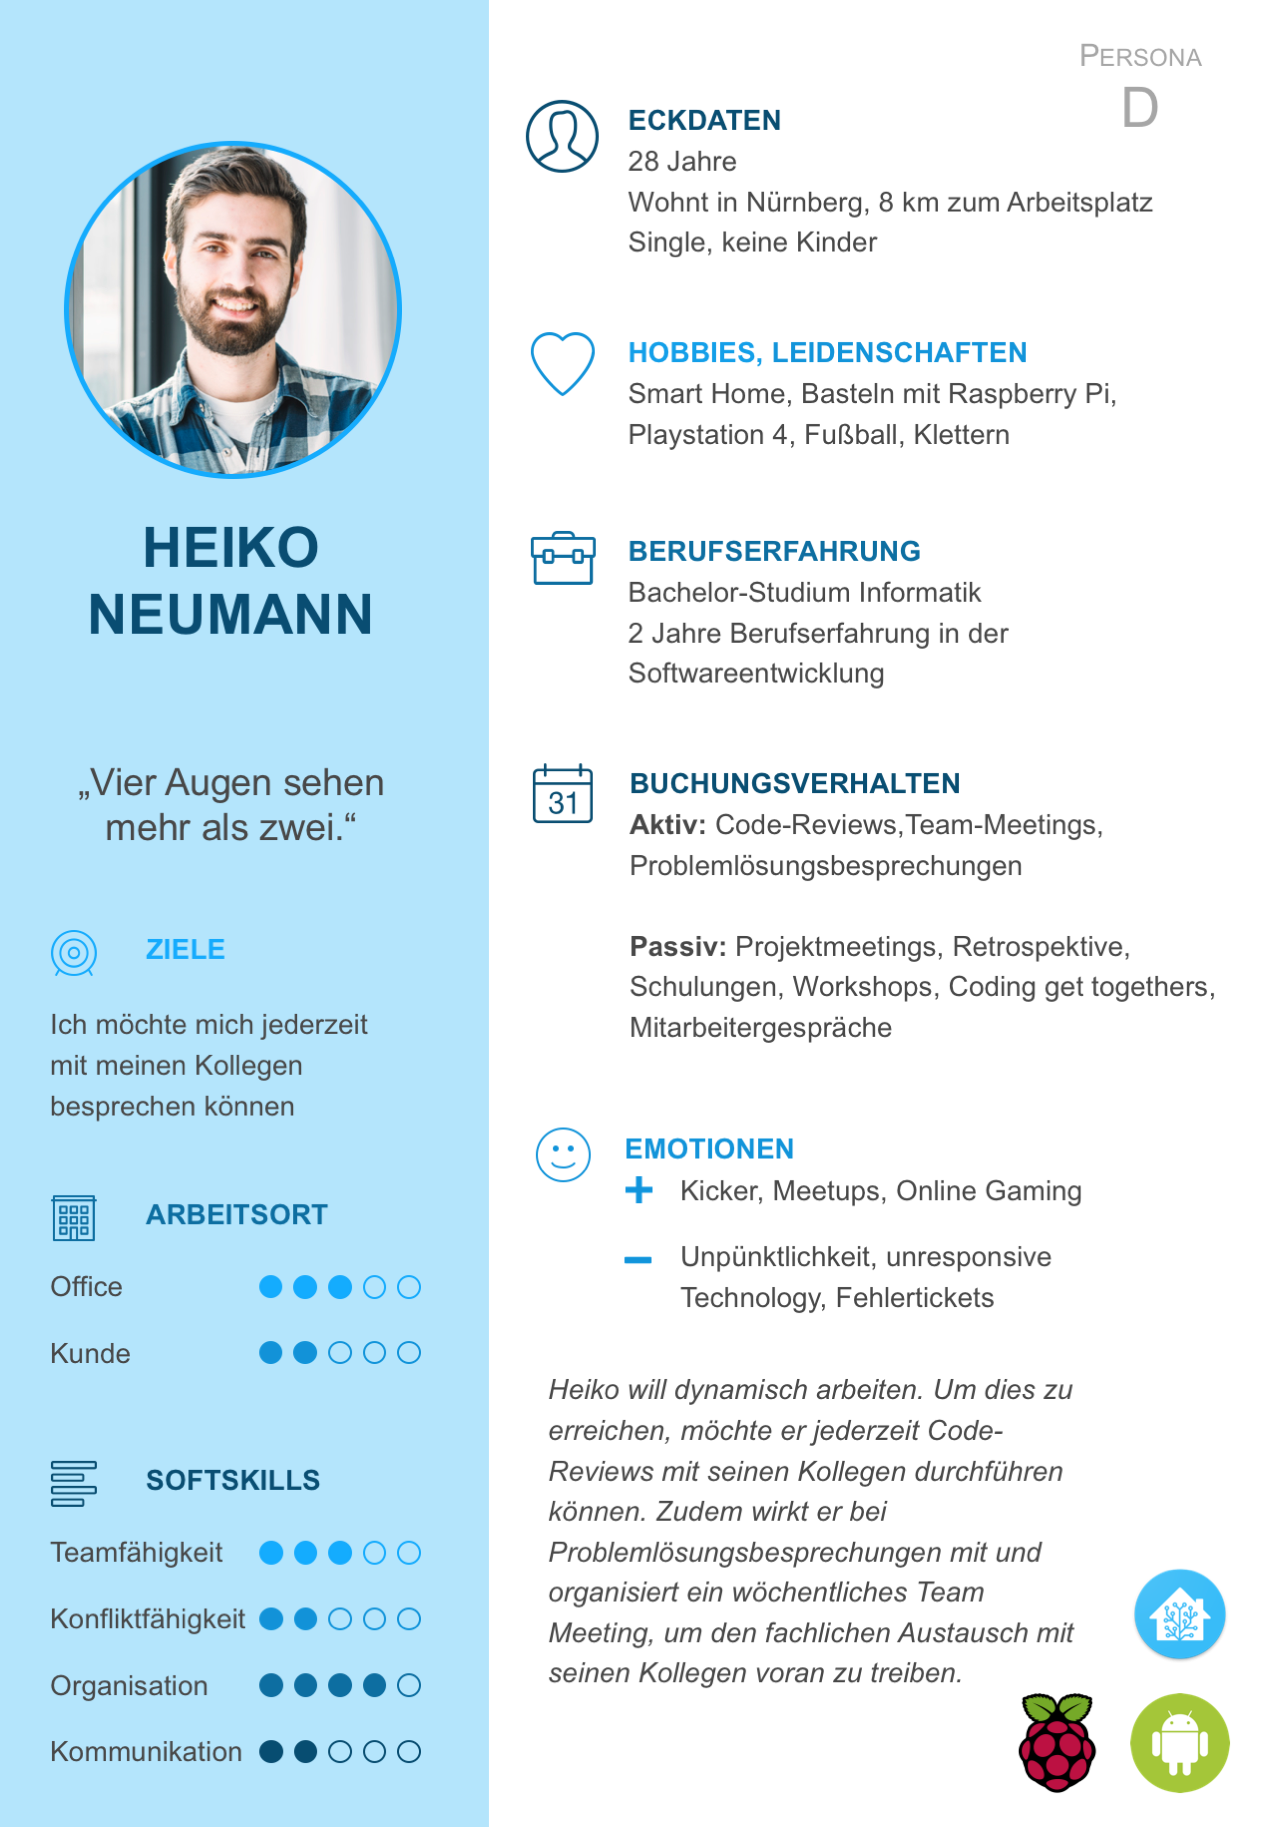
\includegraphics[width=0.9\textwidth]{bilder/anhang/Personae/PersonaD.png}}
    \caption{Persona Heiko Neumann aus dem Bereich \textit{Development}}
    \label{fig:persona-development}
\end{figure}

\begin{figure}[!htb]
    \centering
    \fbox{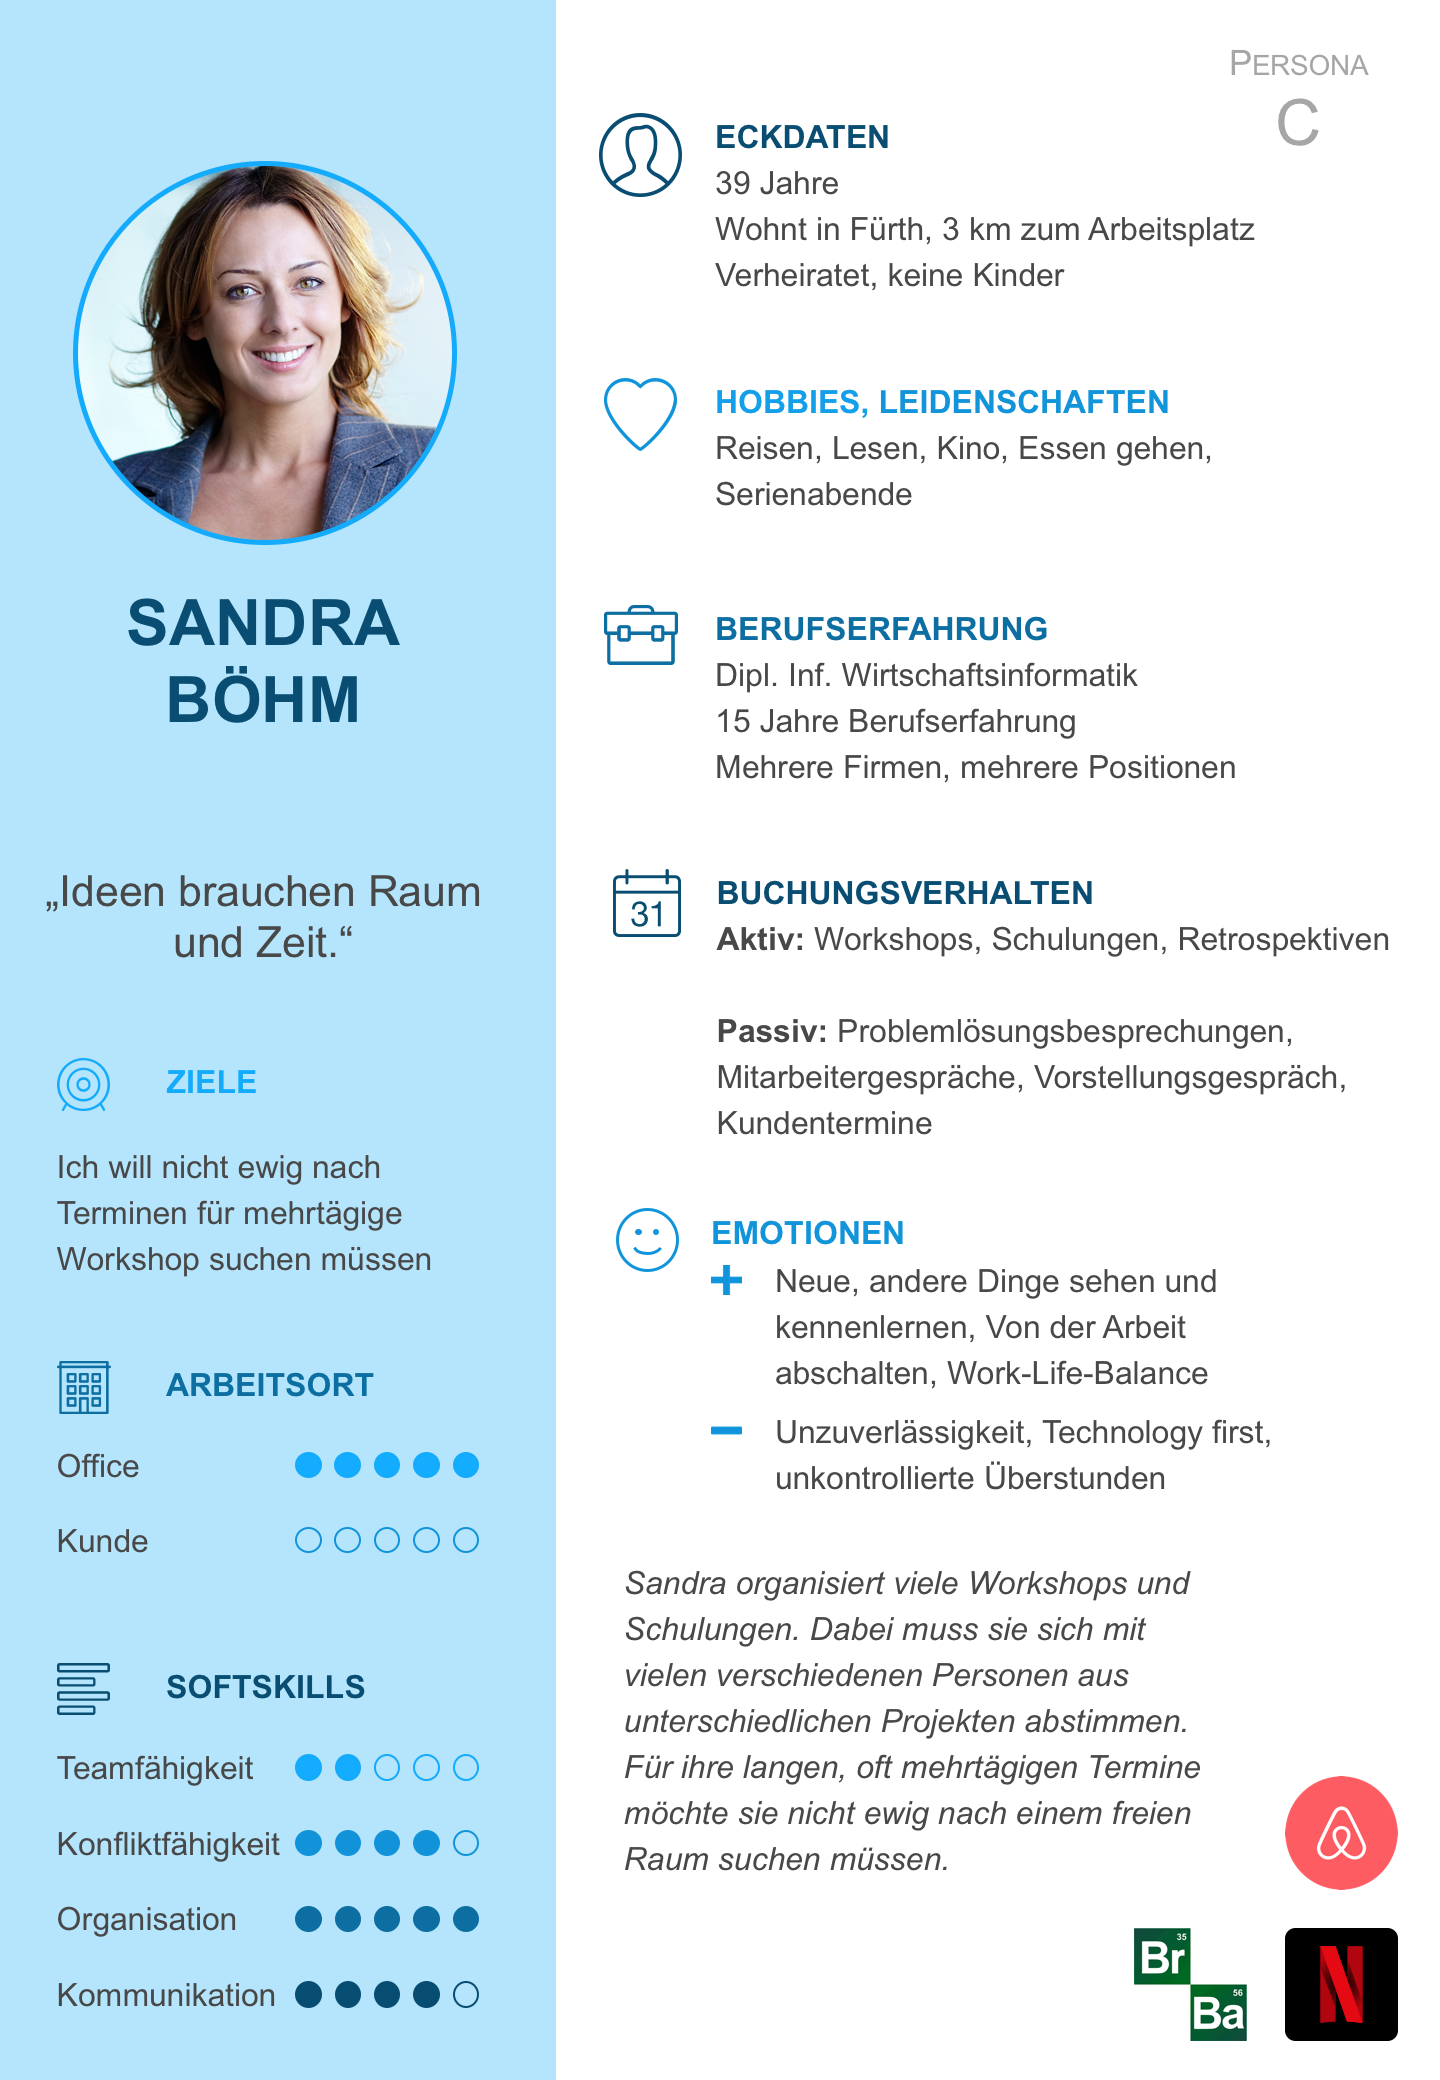
\includegraphics[width=0.9\textwidth]{bilder/anhang/Personae/PersonaC.png}}
    \caption{Persona Sandra Böhm aus dem Bereich \textit{Coaching}}
    \label{fig:persona-coaching}
\end{figure}

\begin{figure}[!htb]
    \centering
    \fbox{
\includegraphics[width=0.9\textwidth]{bilder/anhang/Personae/PersonaHR.png}}
    \caption{Persona Michelle Färber aus dem Bereich \textit{Human Resources}}
    \label{fig:persona-human-resources}
\end{figure}

\begin{figure}[!htb]
    \centering
    \fbox{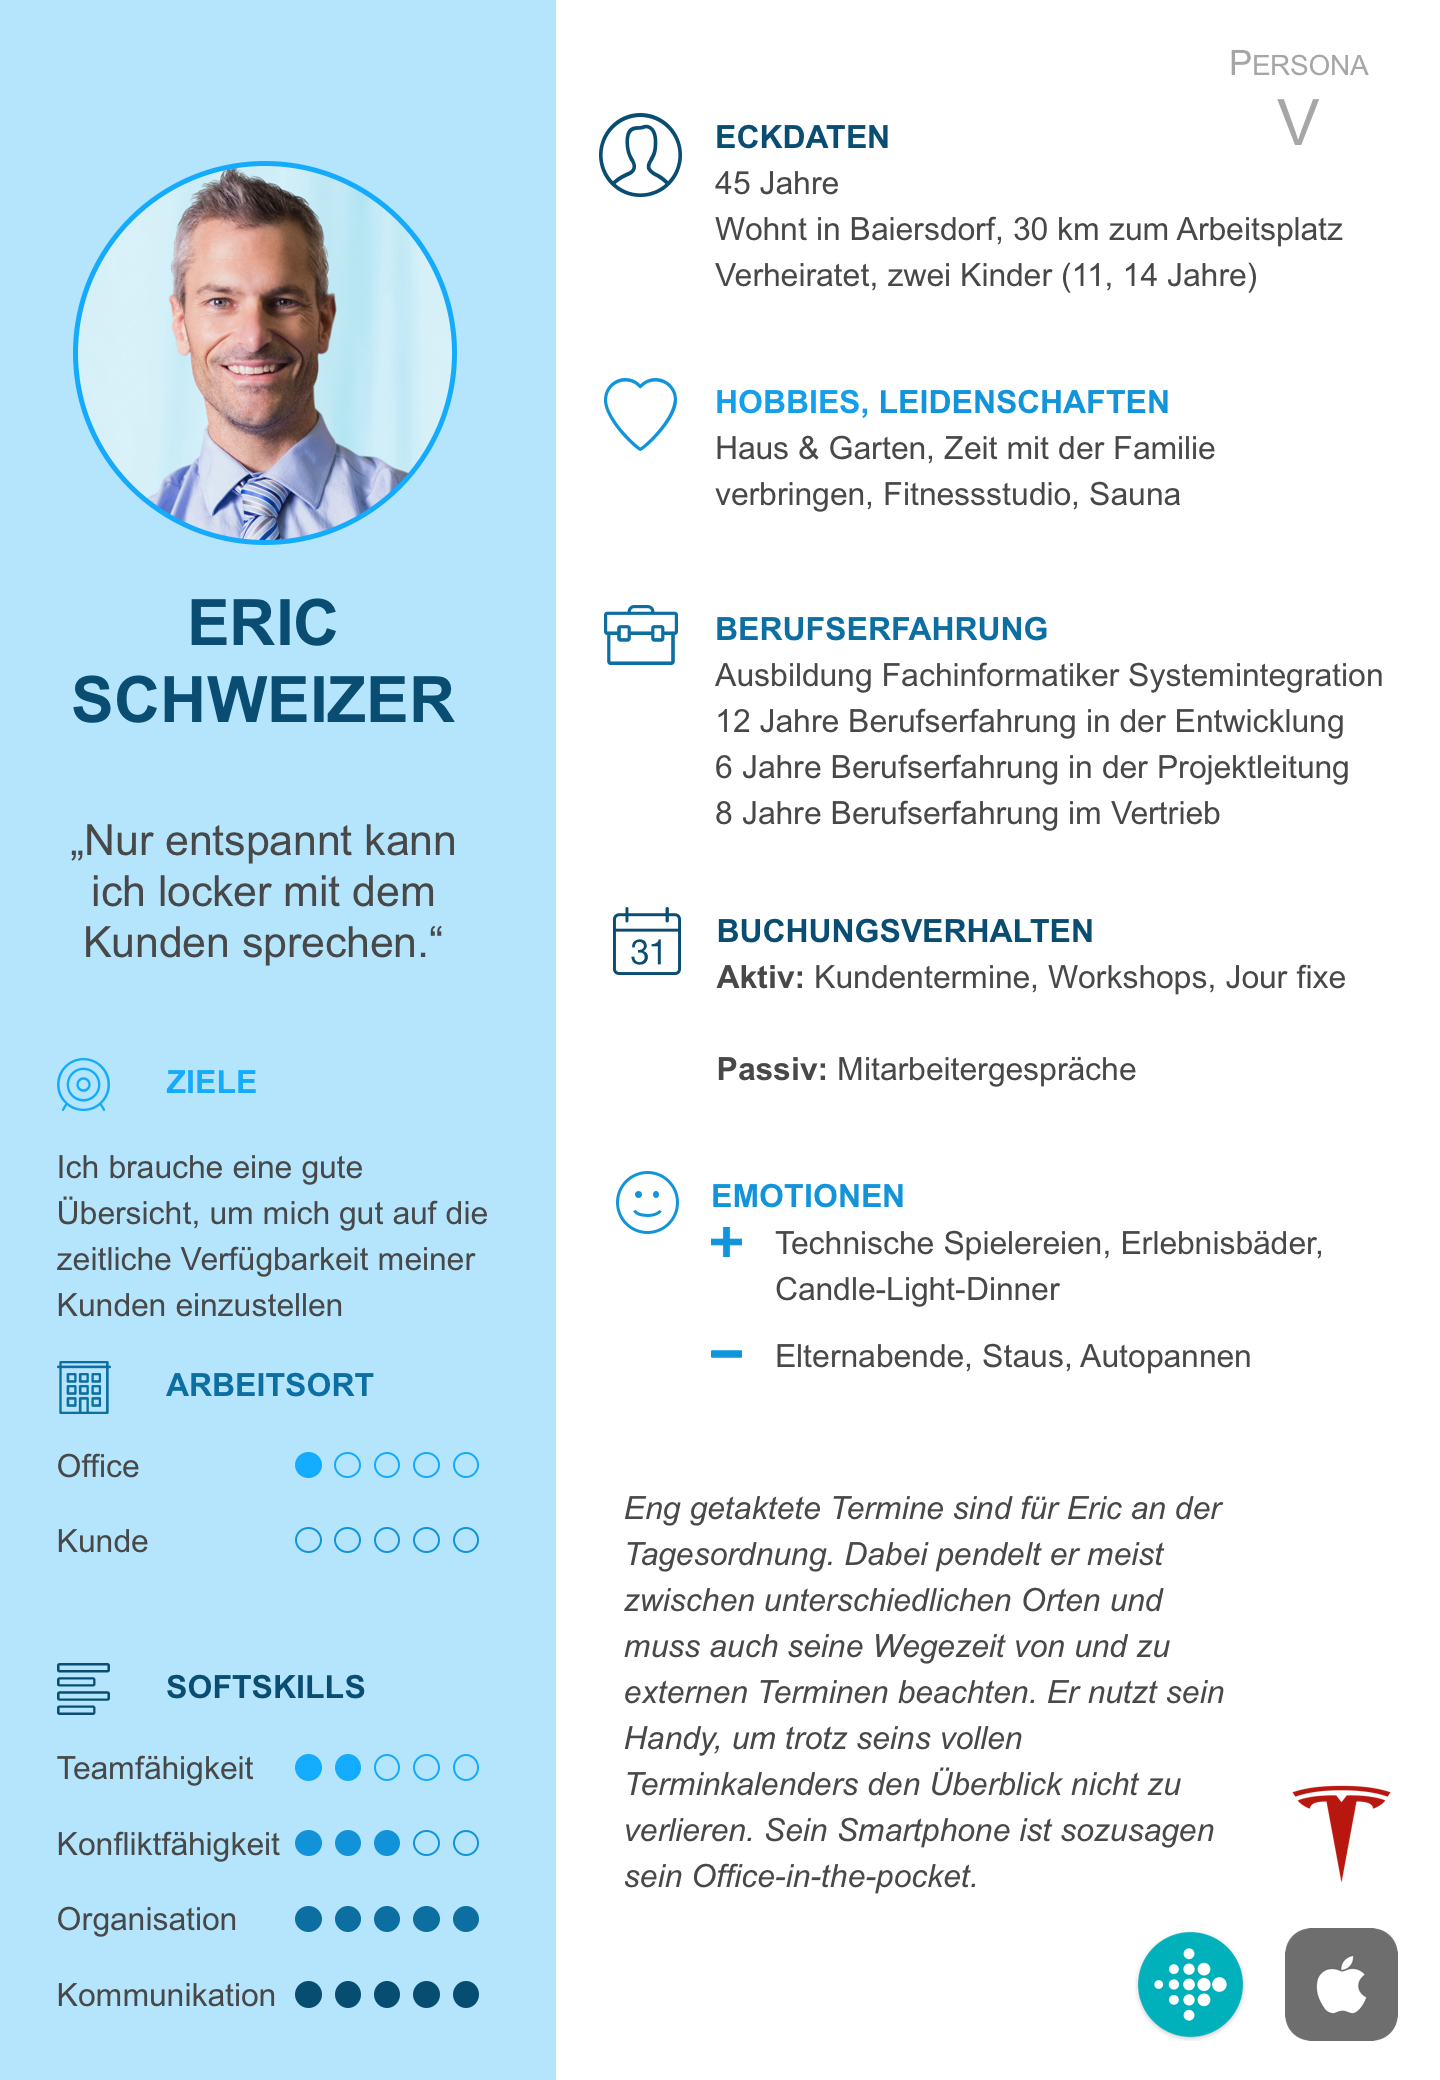
\includegraphics[width=0.9\textwidth]{bilder/anhang/Personae/PersonaV.png}}
    \caption{Persona Eric Schweizer aus dem Bereich \textit{Vertrieb}}
    \label{fig:persona-vertrieb}
\end{figure}

\clearpage

\section{\acs{UI}-Elemente aus dem Prototyping Tool}
\label{sec:anhang-ui-elemente-prototyping}

\begin{figure}[!htb]
    \centering
    \vspace{1.5cm}
    
\includegraphics[width=0.7\textwidth]{bilder/anhang/UIElementsPrototyping/TextMessage.png}
    \caption{\acs{UI}-Element \textit{TextMessage} aus dem Prototyping Tool}
    \label{fig:ui-element-textmessage}
\end{figure}

\begin{figure}[!htb]
    \centering
    \vspace{1.5cm}
    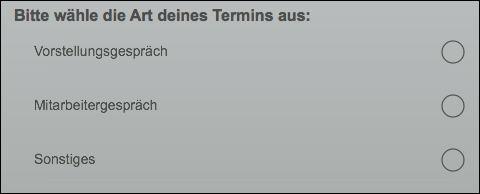
\includegraphics[width=0.7\textwidth]{bilder/anhang/UIElementsPrototyping/TypeOfMeeting.png}
    \caption{\acs{UI}-Element \textit{TypeOfMeeting} aus dem Prototyping Tool}
    \label{fig:ui-element-typeofmeeting}
\end{figure}

\begin{figure}[!htb]
    \centering
    \vspace{1.5cm}
    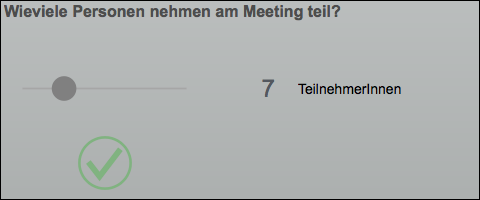
\includegraphics[width=0.7\textwidth]{bilder/anhang/UIElementsPrototyping/SliderParticipants.png}
    \caption{\acs{UI}-Element \textit{SliderParticipants} aus dem Prototyping Tool}
    \label{fig:ui-element-sliderparticipants}
\end{figure}

\begin{figure}[!htb]
    \centering
    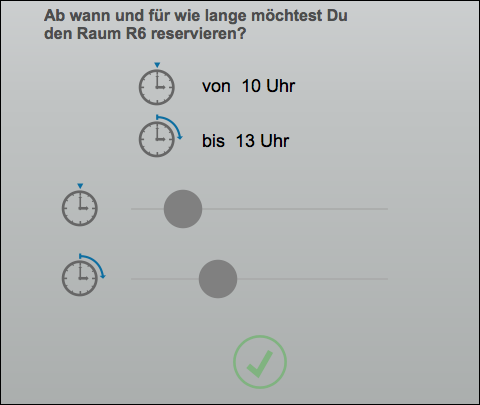
\includegraphics[width=0.6\textwidth]{bilder/anhang/UIElementsPrototyping/SliderStartEndTime.png}
    \caption{\acs{UI}-Element \textit{SliderStartEndTime} aus dem Prototyping Tool}
    \label{fig:ui-element-sliderstartendtime}
\end{figure}

\begin{figure}[!htb]
    \centering
    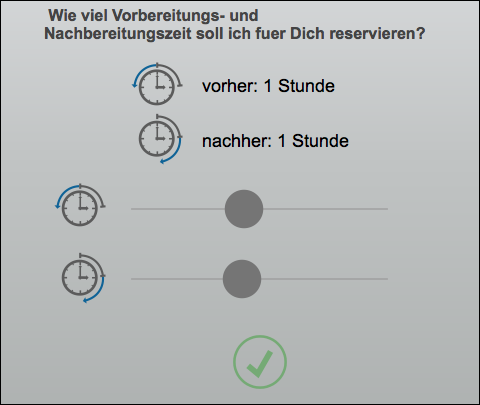
\includegraphics[width=0.6\textwidth]{bilder/anhang/UIElementsPrototyping/SliderTimeBuffer.png}
    \caption{\acs{UI}-Element \textit{SliderTimeBuffer} aus dem Prototyping Tool}
    \label{fig:ui-element-slidertimebuffer}
\end{figure}

\begin{figure}[!htb]
    \centering
    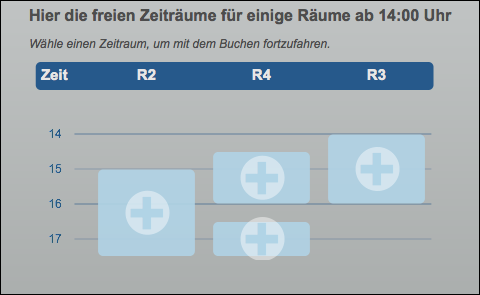
\includegraphics[width=0.7\textwidth]{bilder/anhang/UIElementsPrototyping/CalendarView.png}
    \caption{\acs{UI}-Element \textit{CalendarView} aus dem Prototyping Tool}
    \label{fig:ui-element-calendarview}
\end{figure}

\begin{figure}[!htb]
    \centering
    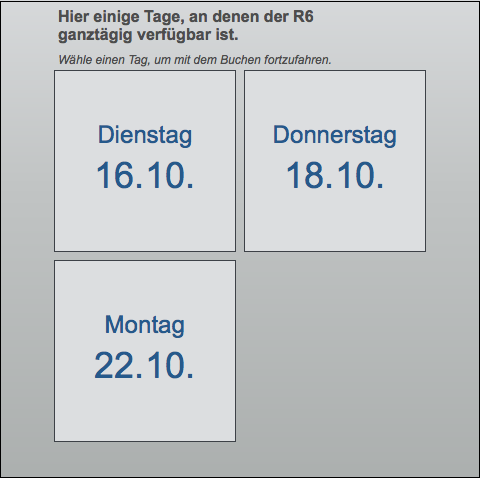
\includegraphics[width=0.6\textwidth]{bilder/anhang/UIElementsPrototyping/CollectionViewDates.png}
    \caption{\acs{UI}-Element \textit{CollectionViewDates} aus dem Prototyping Tool}
    \label{fig:ui-element-collectionviewdates}
\end{figure}

\begin{figure}[!htb]
    \centering
    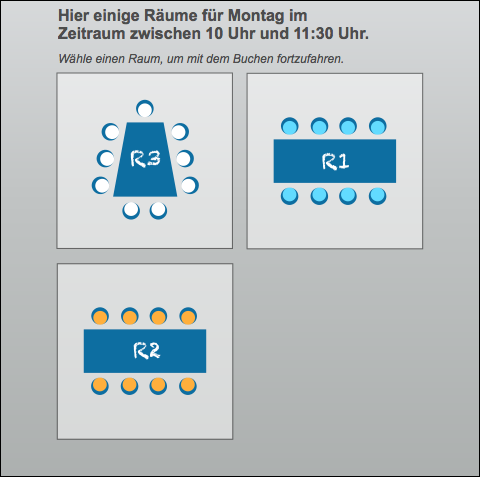
\includegraphics[width=0.6\textwidth]{bilder/anhang/UIElementsPrototyping/CollectionViewRooms.png}
    \caption{\acs{UI}-Element \textit{CollectionViewRooms} aus dem Prototyping Tool}
    \label{fig:ui-element-collectionviewrooms}
\end{figure}

\begin{figure}[!htb]
    \centering
    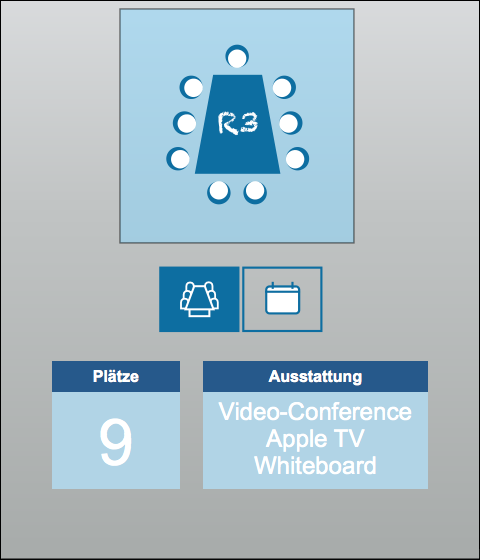
\includegraphics[width=0.6\textwidth]{bilder/anhang/UIElementsPrototyping/DetailView.png}
    \caption{\acs{UI}-Element \textit{DetailView} aus dem Prototyping Tool}
    \label{fig:ui-element-detailview}
\end{figure}

\begin{figure}[!htb]
    \centering
    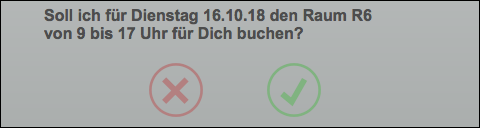
\includegraphics[width=0.7\textwidth]{bilder/anhang/UIElementsPrototyping/ConfirmBookingYesNo.png}
    \caption{\acs{UI}-Element \textit{ConfirmBooking} aus dem Prototyping Tool}
    \label{fig:ui-element-confirmbooking}
\end{figure}

\begin{figure}[!htb]
    \centering
    
\includegraphics[width=0.6\textwidth]{bilder/anhang/UIElementsPrototyping/Certificate.png}
    \caption{\acs{UI}-Element \textit{Certificate} aus dem Prototyping Tool}
    \label{fig:ui-element-certificate}
\end{figure}

\begin{figure}[!htb]
    \centering
    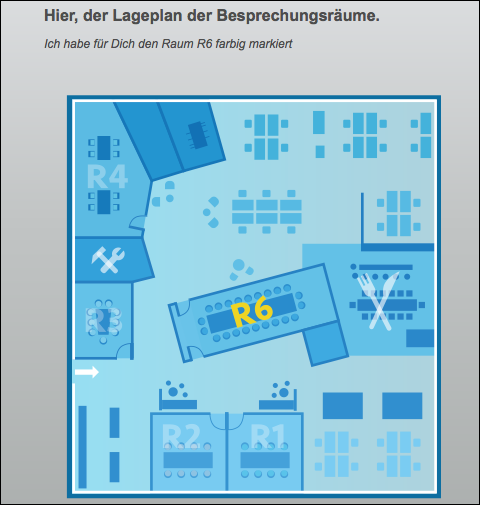
\includegraphics[width=0.6\textwidth]{bilder/anhang/UIElementsPrototyping/RoomMap.png}
    \caption{\acs{UI}-Element \textit{RoomMap} aus dem Prototyping Tool}
    \label{fig:ui-element-roommap}
\end{figure}

\section{Einverständniserklärung zum User Test}
\label{sec:anhang-einverstaendnis-user-test}

Die folgende Einverständniserklärung wird den Teilnehmern vor der Durchführung des
User Tests zur Unterschrift vorgelegt.

\textbf{Usability-Test zur Erfassung von Erfahrungen und Erwartungen in Hinblick auf die Nutzung eines Chatbots um einen Raum zu buchen}

Im Rahmen einer Masterarbeit an der Technischen Hochschule Nürnberg in Zusammenarbeit mit der \adorsys\ beschäftigen wir uns mit dem Design, der Bedienung und der Funktionalität eines Chatbots, mit dessen Hilfe Mitarbeiter und Mitarbeiterinnen einen Besprechungsraum reservieren können. Hierbei geht es um:

\begin{itemize}
\item die Benutzerführung für einen entsprechenden Chatbot
\item die Informationen, welche Nutzer von einem solchen Chatbot erwarten 
\item den Kommunikationsstil, den Nutzer erwarten
\end{itemize}

Hierfür führen wir einen Usability-Test mit einem von uns entwickelten Prototyping-Tool durch. Das Ziel ist es, mehr über Erwartungen von potentiellen Anwendern und die von ihnen verwendeten Formulierungen bei Nutzung eines Conversational Interfaces zu erfahren, und diese Erkenntnisse in die Entwicklung des Chatbots einfließen lassen zu können. 

Alle Fragen und Aufgaben in diesem Usability-Test beziehen sich auf die Einstufung und Verbesserung des Chatbots und nicht darauf, die Fähigkeiten und Fertigkeiten der Testperson zu testen. Alle Angaben werden vertraulich behandelt und ausschließlich anonymisiert verarbeitet und archiviert. Weiterhin werden diese Angaben nur im Rahmen der Entwicklung dieses Chatbots und in hierauf bezogene Präsentationen verwendet.

\begin{itemize}
\item Unternehmen: \adorsys\
\item Projektleitung: Steffen Blümm, Technical Lead iOS / CUI
\item Method: Think-Aloud
\item Dauer: 
\item Datum: 
\end{itemize}

\textbf{Einverständniserklärung}

Ich erkläre mich dazu bereit, im Rahmen des oben beschriebenen Projekts an einen Usability-Test teilzunehmen. Ich wurde über die Ziele des Projekts informiert. Ich kann den Test jederzeit abbrechen, weitere Tests ablehnen und meine Einwilligung in eine Aufzeichnung und Niederschrift des Tests jederzeit zurückziehen, ohne dass mir dadurch irgendwelche Nachteile entstehen.

Ich bin damit einverstanden, dass der Test mit einem Aufnahmegerät aufgezeichnet und sodann von den MitarbeiterInnen der adorsys ausgewertet wird. Für die Auswertung des Usability-Tests werden alle Angaben zu meiner Person aus dem Text entfernt und/oder anonymisiert. Mir wurde außerdem versichert, dass der Test in Veröffentlichungen nur in Ausschnitten zitiert wird, um sicherzustellen, dass ich auch durch die Reihenfolge von im Test erwähnten Ereignissen nicht für Dritte erkennbar sein werde. 
\\ \\ \\ \\ \\
Datum, Unterschrift der Testperson

\label{sec:anhang-einverstaendniserklaerung-feedback-ext}

\clearpage

\section{Feedback zum Usability Testessen}
\label{sec:anhang-feedback-ext}

\begin{figure}[!htb]
    \centering
    \fbox{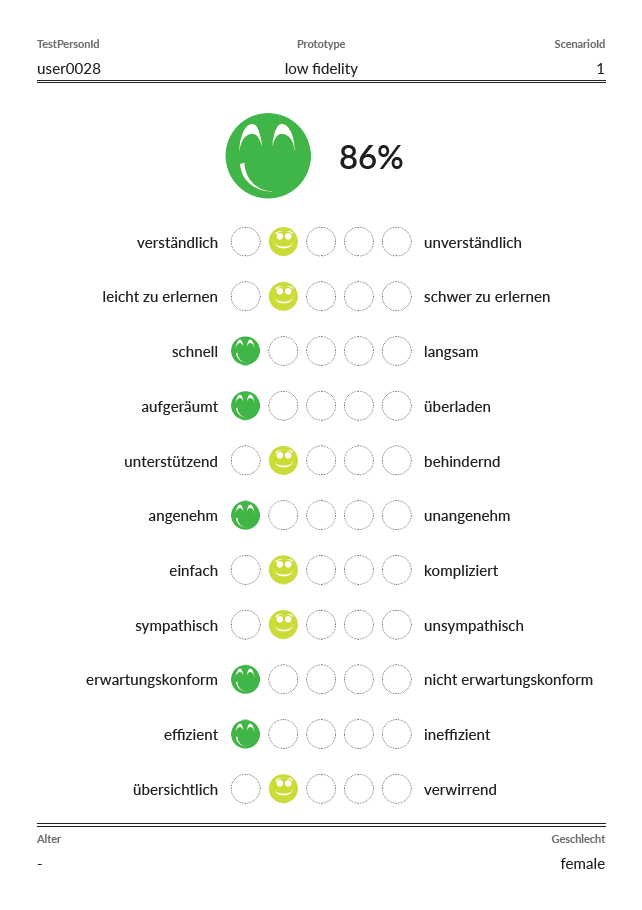
\includegraphics[width=0.9\textwidth]{bilder/anhang/UsabilityTestEssen/user0028-front.png}}
    \caption{Ergebnisse zum Fragebogen von user0028}
    \label{fig:feedback-user0028-front}
\end{figure}

\begin{figure}[!htb]
    \centering
    \fbox{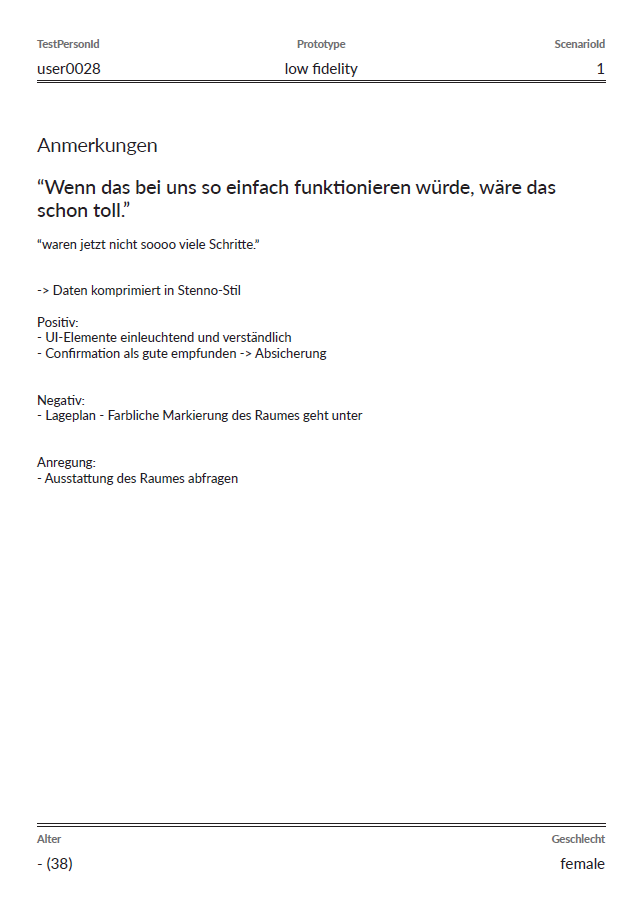
\includegraphics[width=0.9\textwidth]{bilder/anhang/UsabilityTestEssen/user0028-back.png}}
    \caption{Notizen zum Fragebogen von user0028}
    \label{fig:feedback-user0028-back}
\end{figure}

% new user

\begin{figure}[!htb]
    \centering
    \fbox{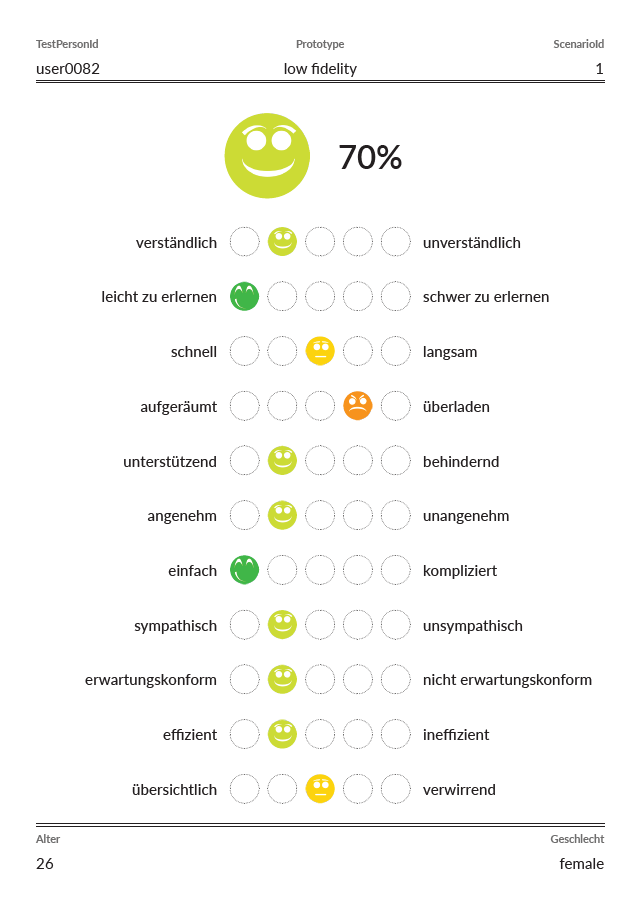
\includegraphics[width=0.9\textwidth]{bilder/anhang/UsabilityTestEssen/user0082-front.png}}
    \caption{Ergebnisse zum Fragebogen von user0082}
    \label{fig:feedback-user0082-front}
\end{figure}

\begin{figure}[!htb]
    \centering
    \fbox{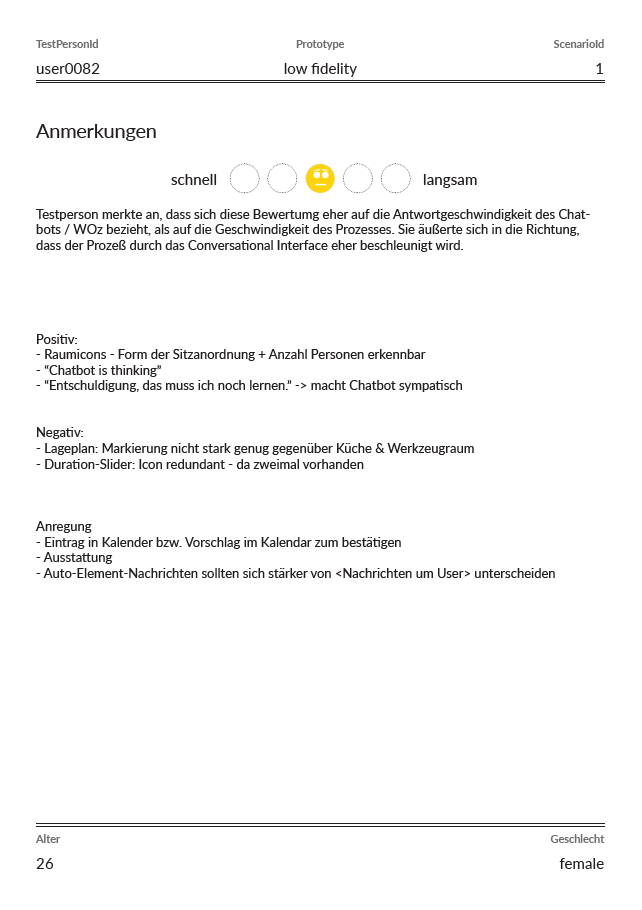
\includegraphics[width=0.9\textwidth]{bilder/anhang/UsabilityTestEssen/user0082-back.png}}
    \caption{Notizen zum Fragebogen von user0082}
    \label{fig:feedback-user0082-back}
\end{figure}

% new user

\begin{figure}[!htb]
    \centering
    \fbox{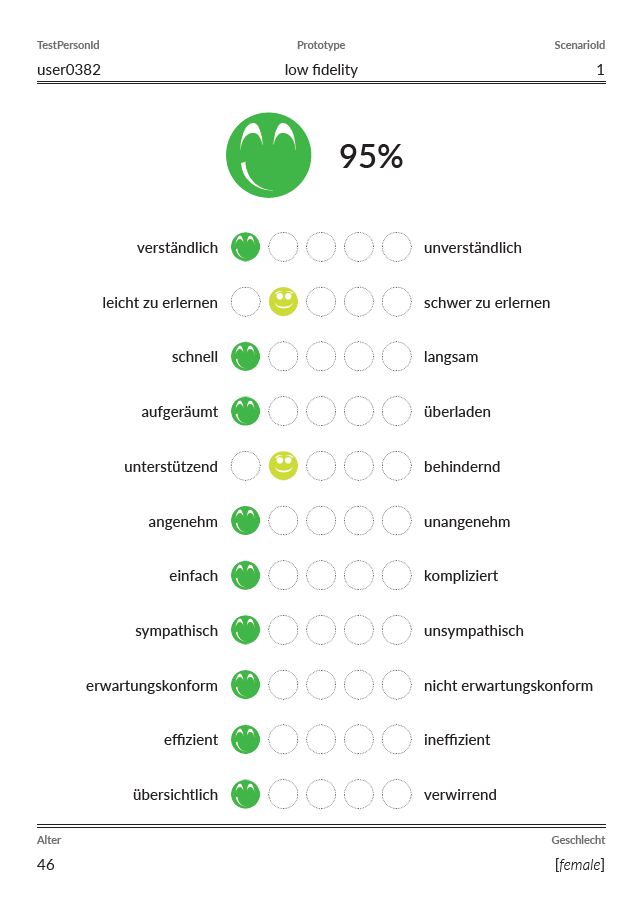
\includegraphics[width=0.9\textwidth]{bilder/anhang/UsabilityTestEssen/user0382-front.png}}
    \caption{Ergebnisse zum Fragebogen von user0382}
    \label{fig:feedback-user0382-front}
\end{figure}

\begin{figure}[!htb]
    \centering
    \fbox{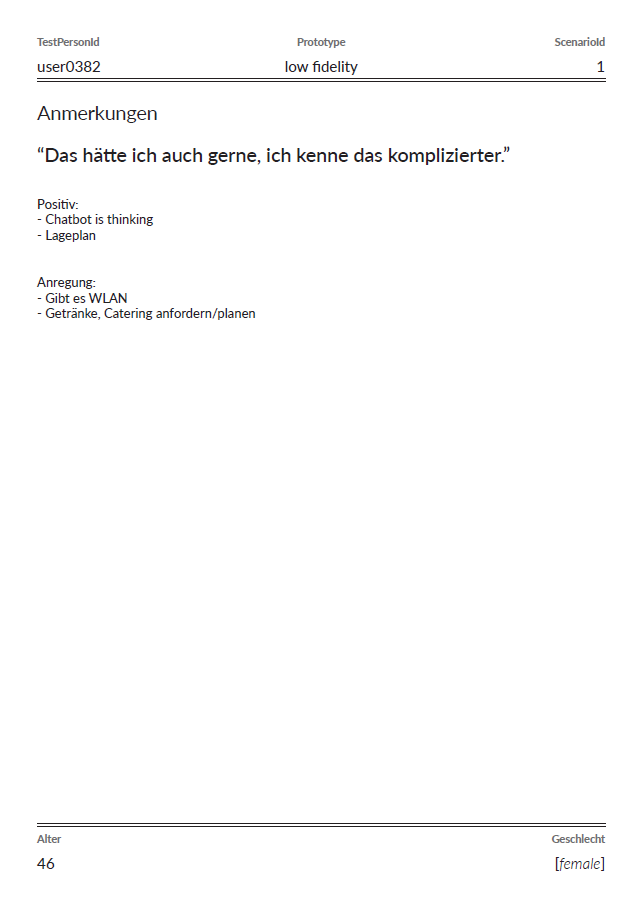
\includegraphics[width=0.9\textwidth]{bilder/anhang/UsabilityTestEssen/user0382-back.png}}
    \caption{Notizen zum Fragebogen von user0382}
    \label{fig:feedback-user0382-back}
\end{figure}

% new user

\begin{figure}[!htb]
    \centering
    \fbox{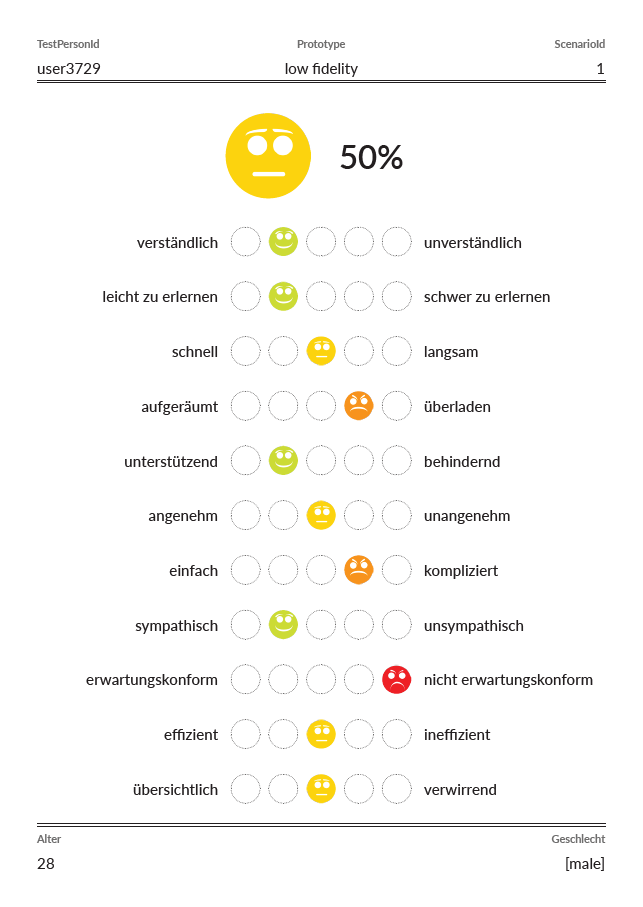
\includegraphics[width=0.9\textwidth]{bilder/anhang/UsabilityTestEssen/user3729-front.png}}
    \caption{Ergebnisse zum Fragebogen von user3729}
    \label{fig:feedback-user3729-front}
\end{figure}

\begin{figure}[!htb]
    \centering
    \fbox{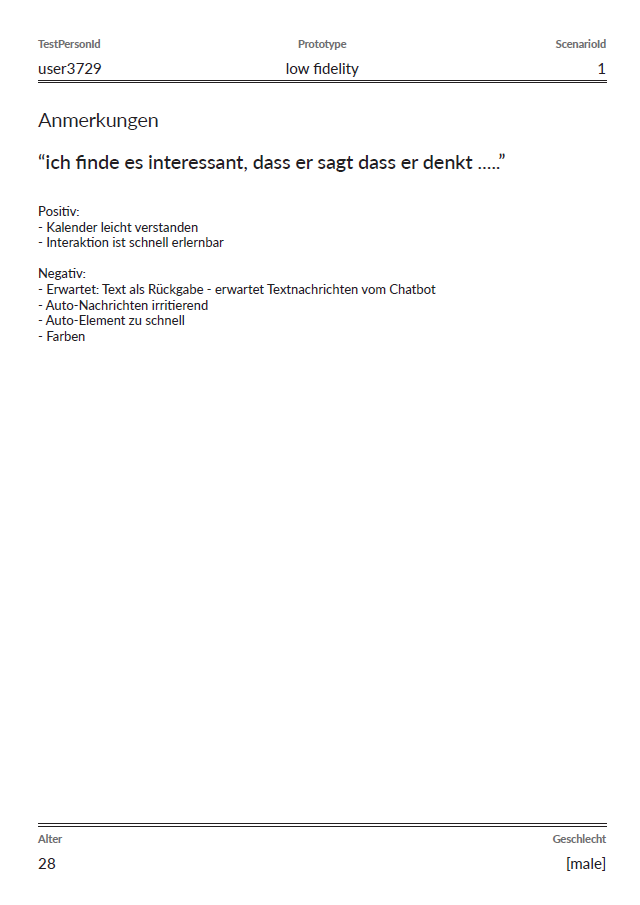
\includegraphics[width=0.9\textwidth]{bilder/anhang/UsabilityTestEssen/user3729-back.png}}
    \caption{Notizen zum Fragebogen von user3729}
    \label{fig:feedback-user3729-back}
\end{figure}

% new user

\begin{figure}[!htb]
    \centering
    \fbox{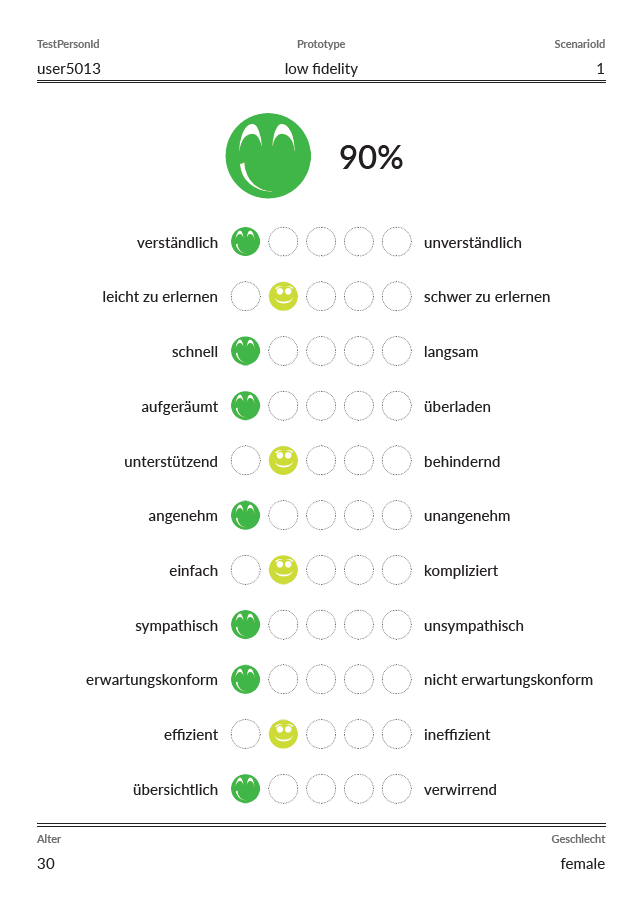
\includegraphics[width=0.9\textwidth]{bilder/anhang/UsabilityTestEssen/user5013-front.png}}
    \caption{Ergebnisse zum Fragebogen von user5013}
    \label{fig:feedback-user5013-front}
\end{figure}

\begin{figure}[!htb]
    \centering
    \fbox{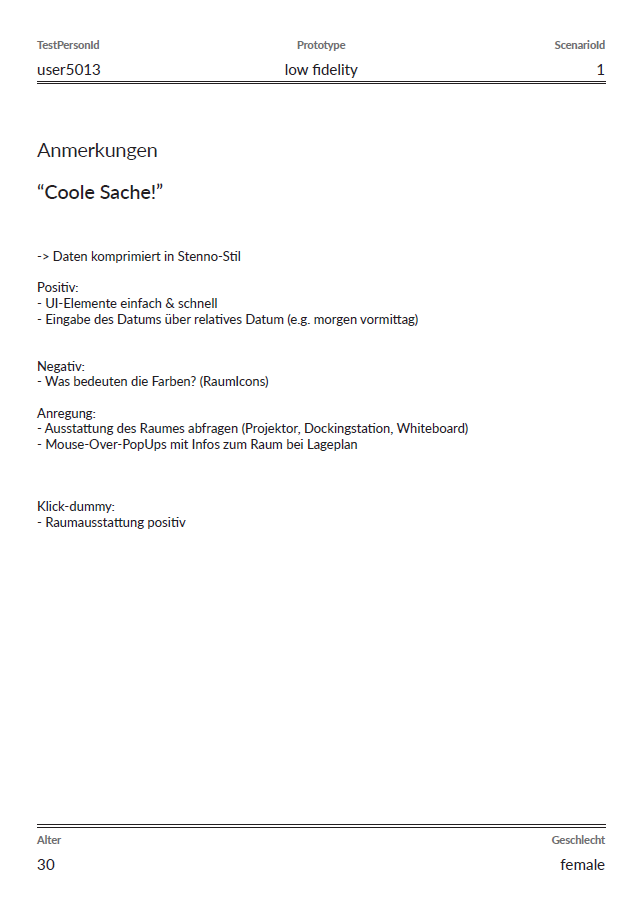
\includegraphics[width=0.9\textwidth]{bilder/anhang/UsabilityTestEssen/user5013-back.png}}
    \caption{Notizen zum Fragebogen von user5013}
    \label{fig:feedback-user5013-back}
\end{figure}

% new user

\begin{figure}[!htb]
    \centering
    \fbox{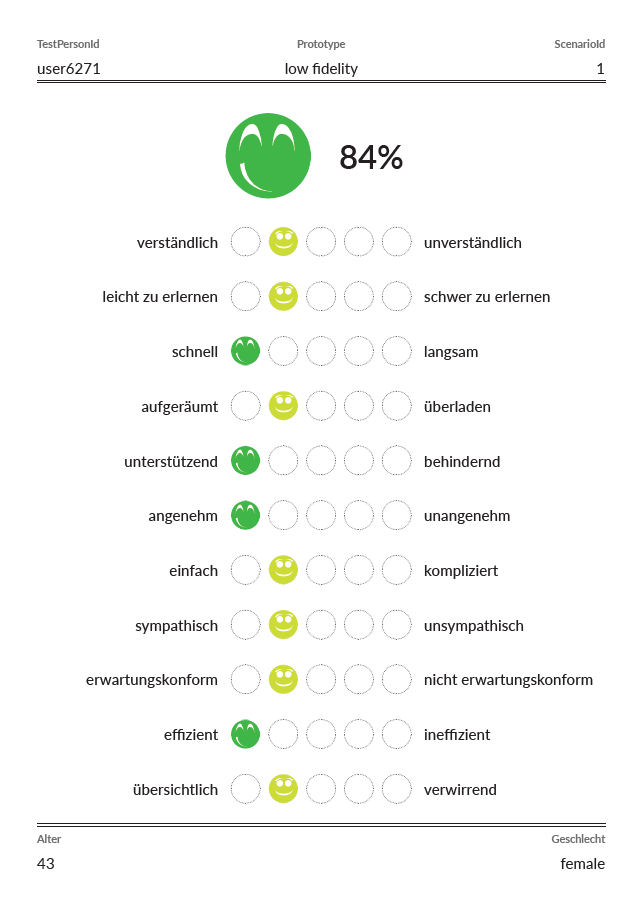
\includegraphics[width=0.9\textwidth]{bilder/anhang/UsabilityTestEssen/user6271-front.png}}
    \caption{Ergebnisse zum Fragebogen von user6271}
    \label{fig:feedback-user6271-front}
\end{figure}

\begin{figure}[!htb]
    \centering
    \fbox{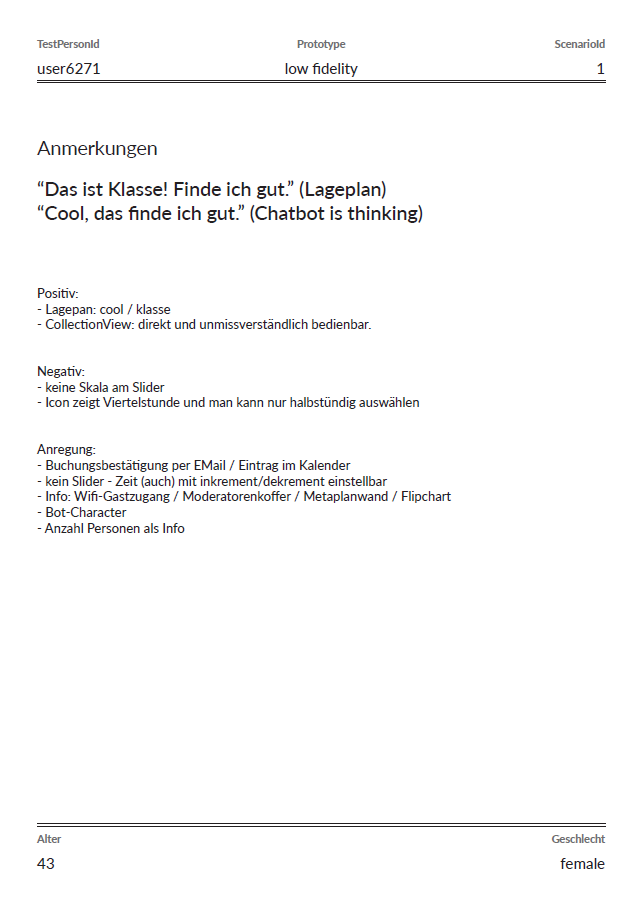
\includegraphics[width=0.9\textwidth]{bilder/anhang/UsabilityTestEssen/user6271-back.png}}
    \caption{Notizen zum Fragebogen von user6271}
    \label{fig:feedback-user6271-back}
\end{figure}

\clearpage

\section{Feedback zum User Test}
\label{sec:anhang-feedback-user-tests}

\begin{figure}[!htb]
    \centering
    \fbox{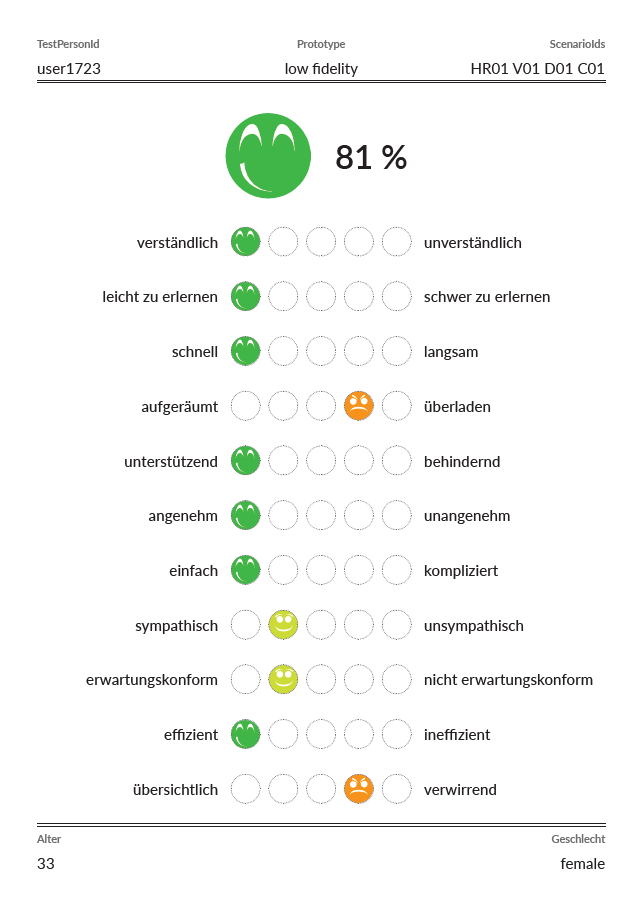
\includegraphics[width=0.9\textwidth]{bilder/anhang/UserTestAdorsys/user1723-front.png}}
    \caption{Ergebnisse zum Fragebogen von user1723}
    \label{fig:feedback-user1723-front}
\end{figure}

\begin{figure}[!htb]
    \centering
    \fbox{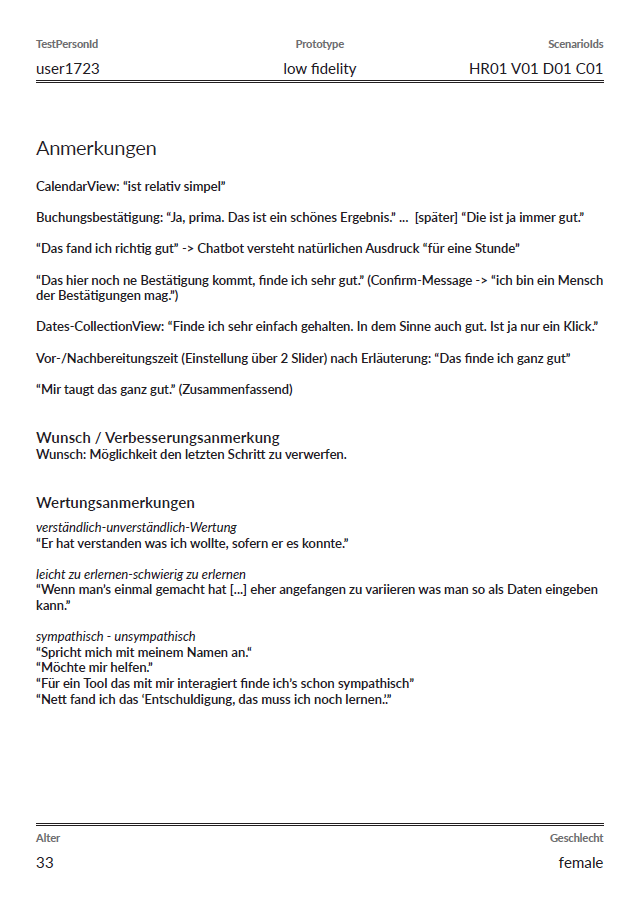
\includegraphics[width=0.9\textwidth]{bilder/anhang/UserTestAdorsys/user1723-back.png}}
    \caption{Notizen zum Fragebogen von user1723}
    \label{fig:feedback-user1723-back}
\end{figure}

% new user

\begin{figure}[!htb]
    \centering
    \fbox{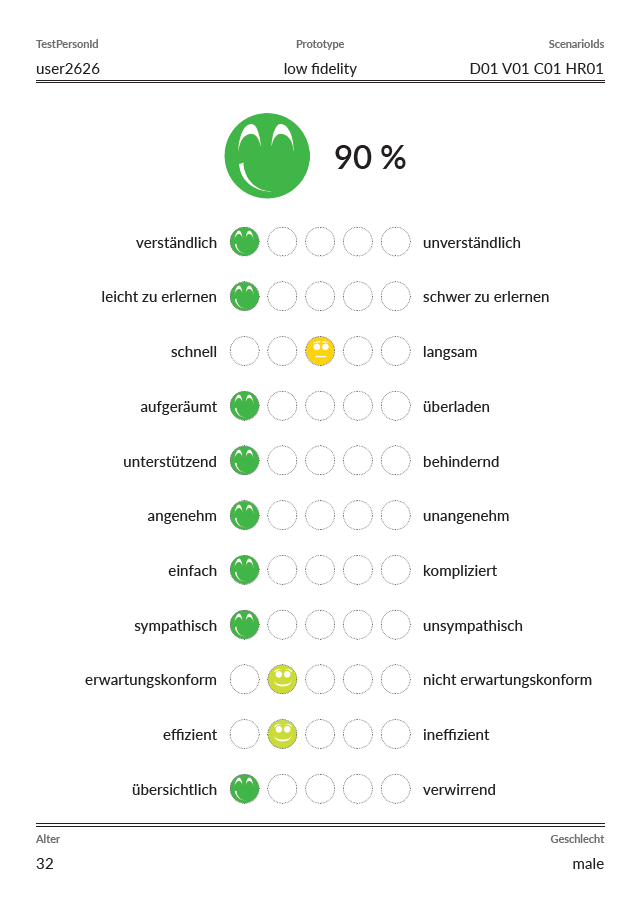
\includegraphics[width=0.9\textwidth]{bilder/anhang/UserTestAdorsys/user2626-front.png}}
    \caption{Ergebnisse zum Fragebogen von user2626}
    \label{fig:feedback-user2626-front}
\end{figure}

\begin{figure}[!htb]
    \centering
    \fbox{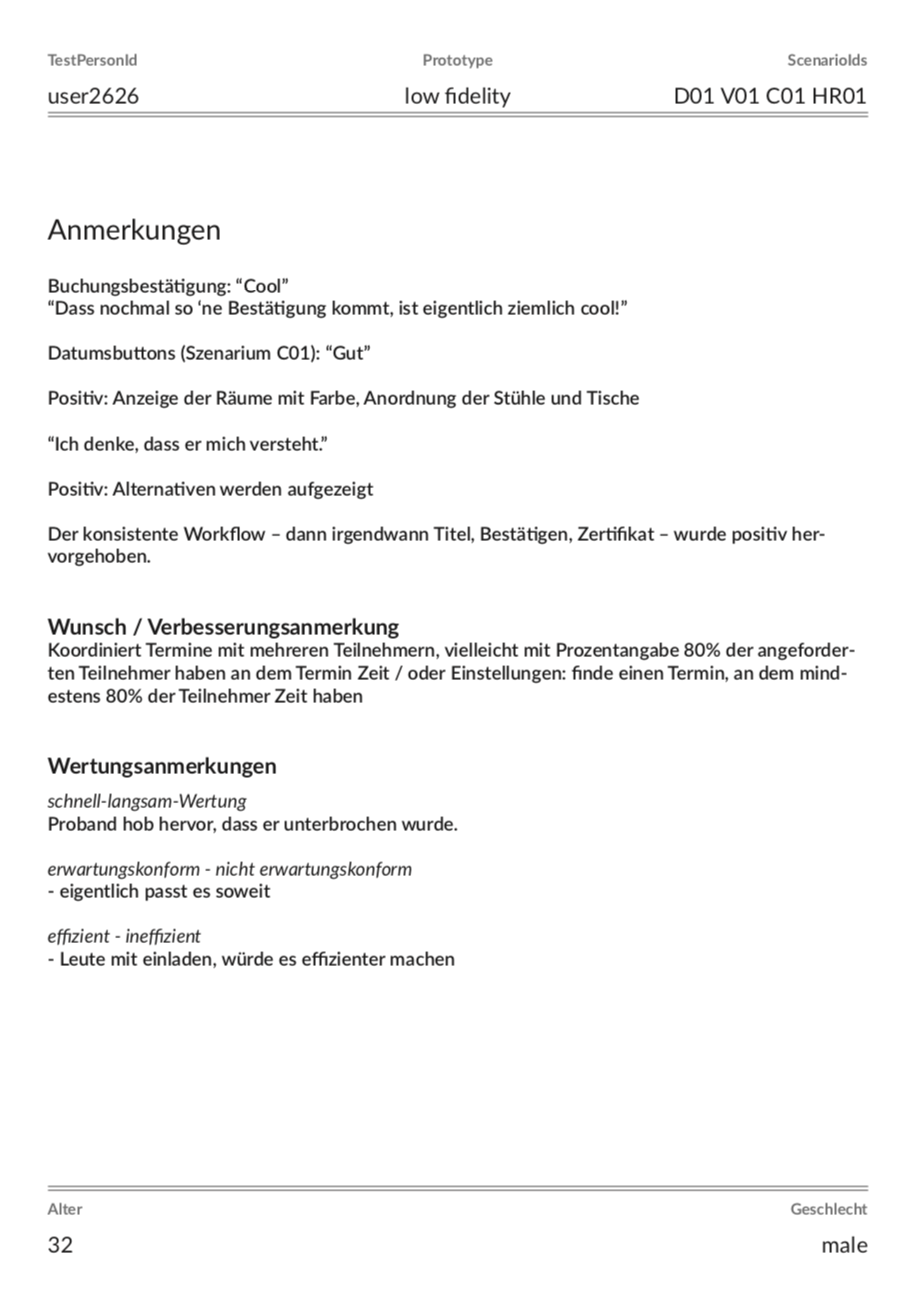
\includegraphics[width=0.9\textwidth]{bilder/anhang/UserTestAdorsys/user2626-back.png}}
    \caption{Notizen zum Fragebogen von user2626}
    \label{fig:feedback-user2626-back}
\end{figure}

% new user

\begin{figure}[!htb]
    \centering
    \fbox{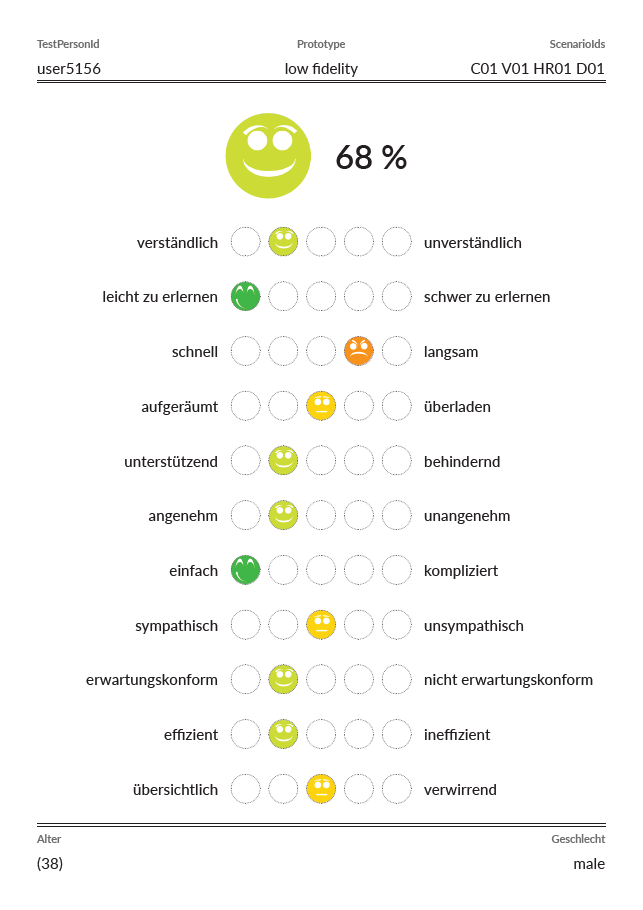
\includegraphics[width=0.9\textwidth]{bilder/anhang/UserTestAdorsys/user5156-front.png}}
    \caption{Ergebnisse zum Fragebogen von user5156}
    \label{fig:feedback-user5156-front}
\end{figure}

\begin{figure}[!htb]
    \centering
    \fbox{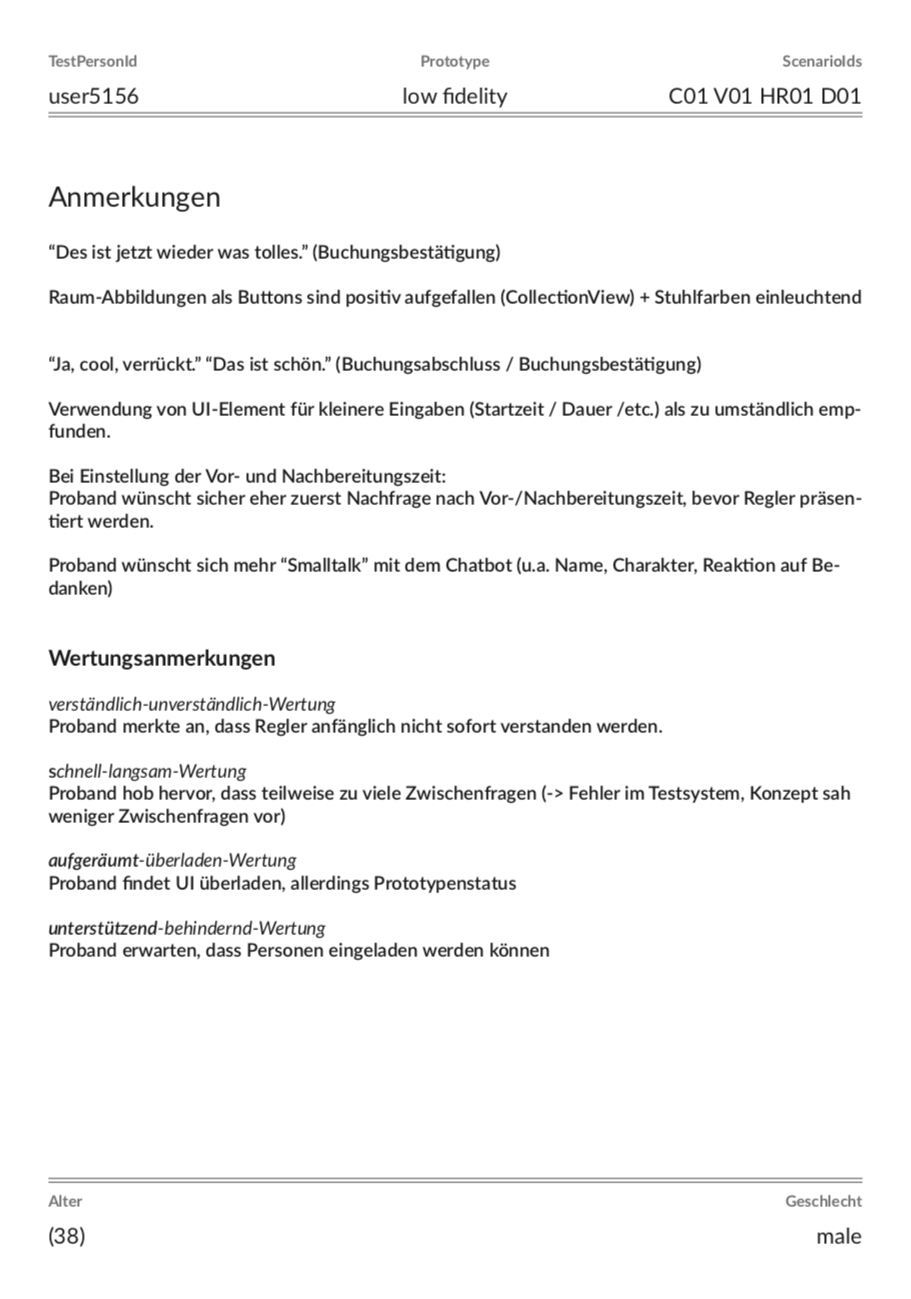
\includegraphics[width=0.9\textwidth]{bilder/anhang/UserTestAdorsys/user5156-back.png}}
    \caption{Notizen zum Fragebogen von user5156}
    \label{fig:feedback-user5156-back}
\end{figure}

% new user

\begin{figure}[!htb]
    \centering
    \fbox{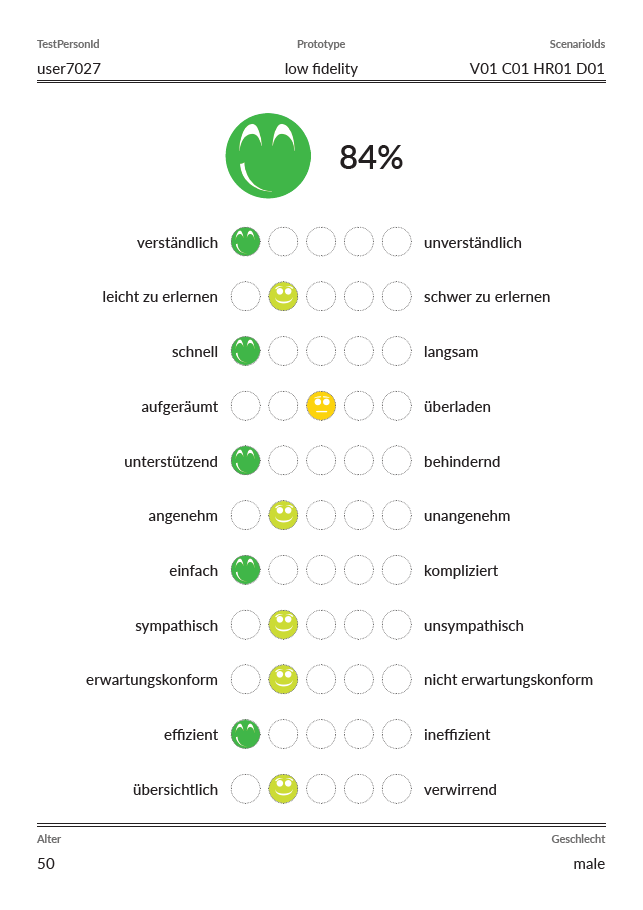
\includegraphics[width=0.9\textwidth]{bilder/anhang/UserTestAdorsys/user7027-front.png}}
    \caption{Ergebnisse zum Fragebogen von user7027}
    \label{fig:feedback-user7027-front}
\end{figure}

\begin{figure}[!htb]
    \centering
    \fbox{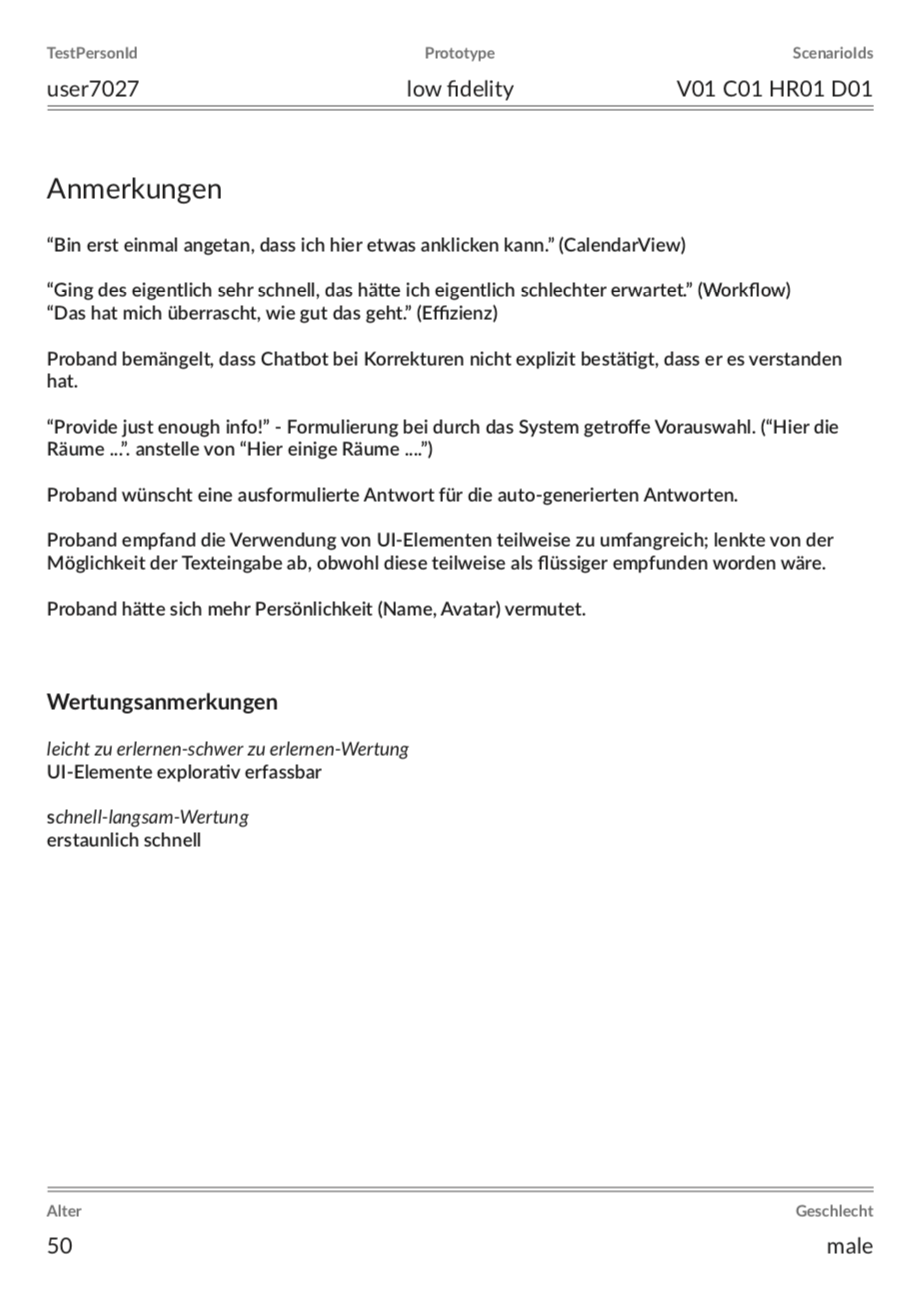
\includegraphics[width=0.9\textwidth]{bilder/anhang/UserTestAdorsys/user7027-back.png}}
    \caption{Notizen zum Fragebogen von user7027}
    \label{fig:feedback-user7027-back}
\end{figure}

% new user

\begin{figure}[!htb]
    \centering
    \fbox{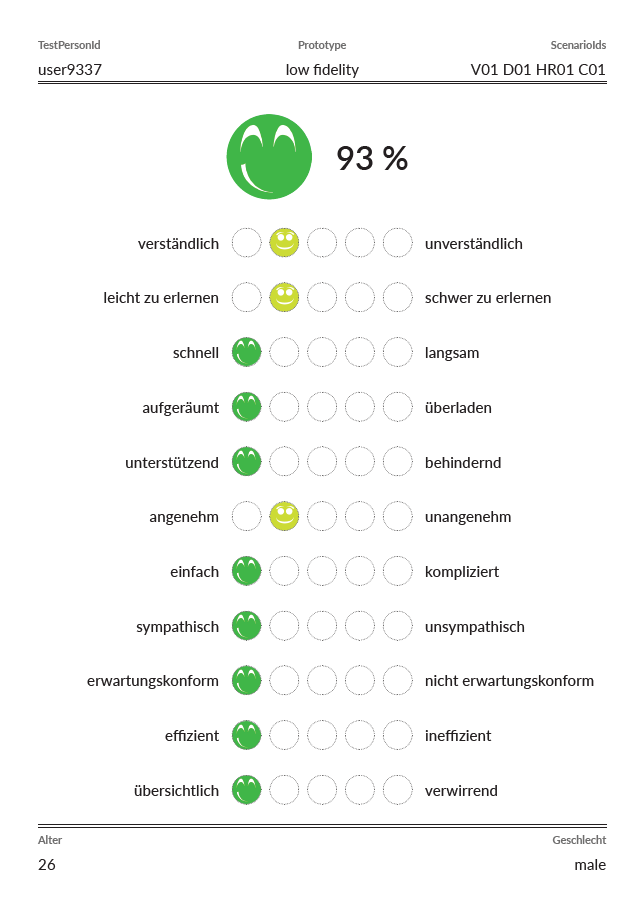
\includegraphics[width=0.9\textwidth]{bilder/anhang/UserTestAdorsys/user9337-front.png}}
    \caption{Ergebnisse zum Fragebogen von user9337}
    \label{fig:feedback-user9337-front}
\end{figure}

\begin{figure}[!htb]
    \centering
    \fbox{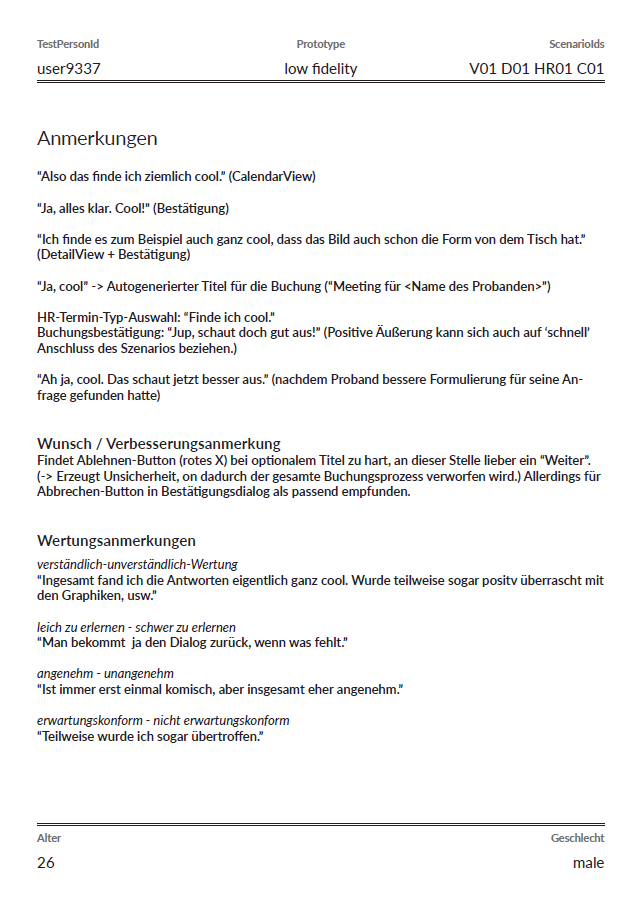
\includegraphics[width=0.9\textwidth]{bilder/anhang/UserTestAdorsys/user9337-back.png}}
    \caption{Notizen zum Fragebogen von user9337}
    \label{fig:feedback-user9337-back}
\end{figure}

% new user

\begin{figure}[!htb]
    \centering
    \fbox{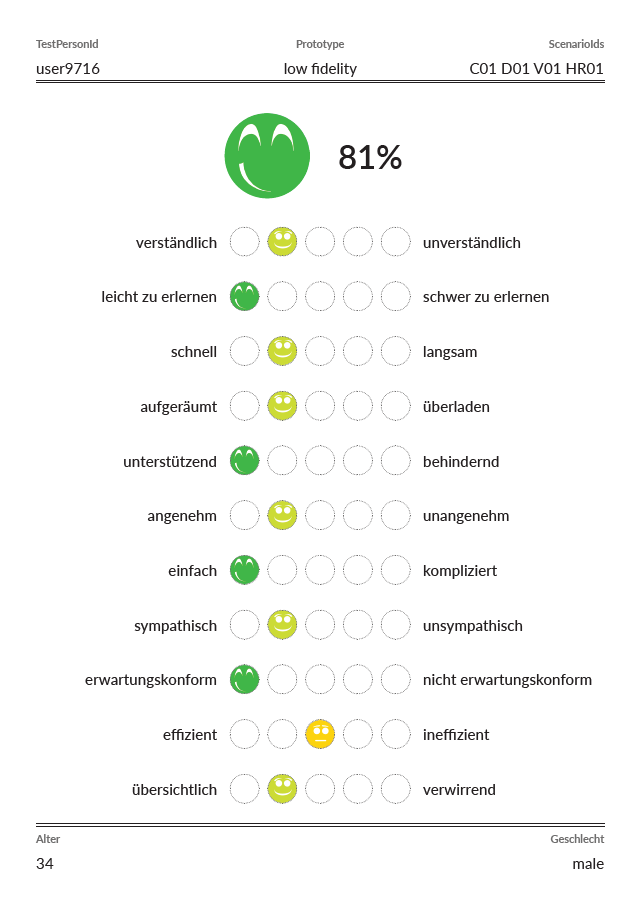
\includegraphics[width=0.9\textwidth]{bilder/anhang/UserTestAdorsys/user9716-front.png}}
    \caption{Ergebnisse zum Fragebogen von user9716}
    \label{fig:feedback-user9716-front}
\end{figure}

\begin{figure}[!htb]
    \centering
    \fbox{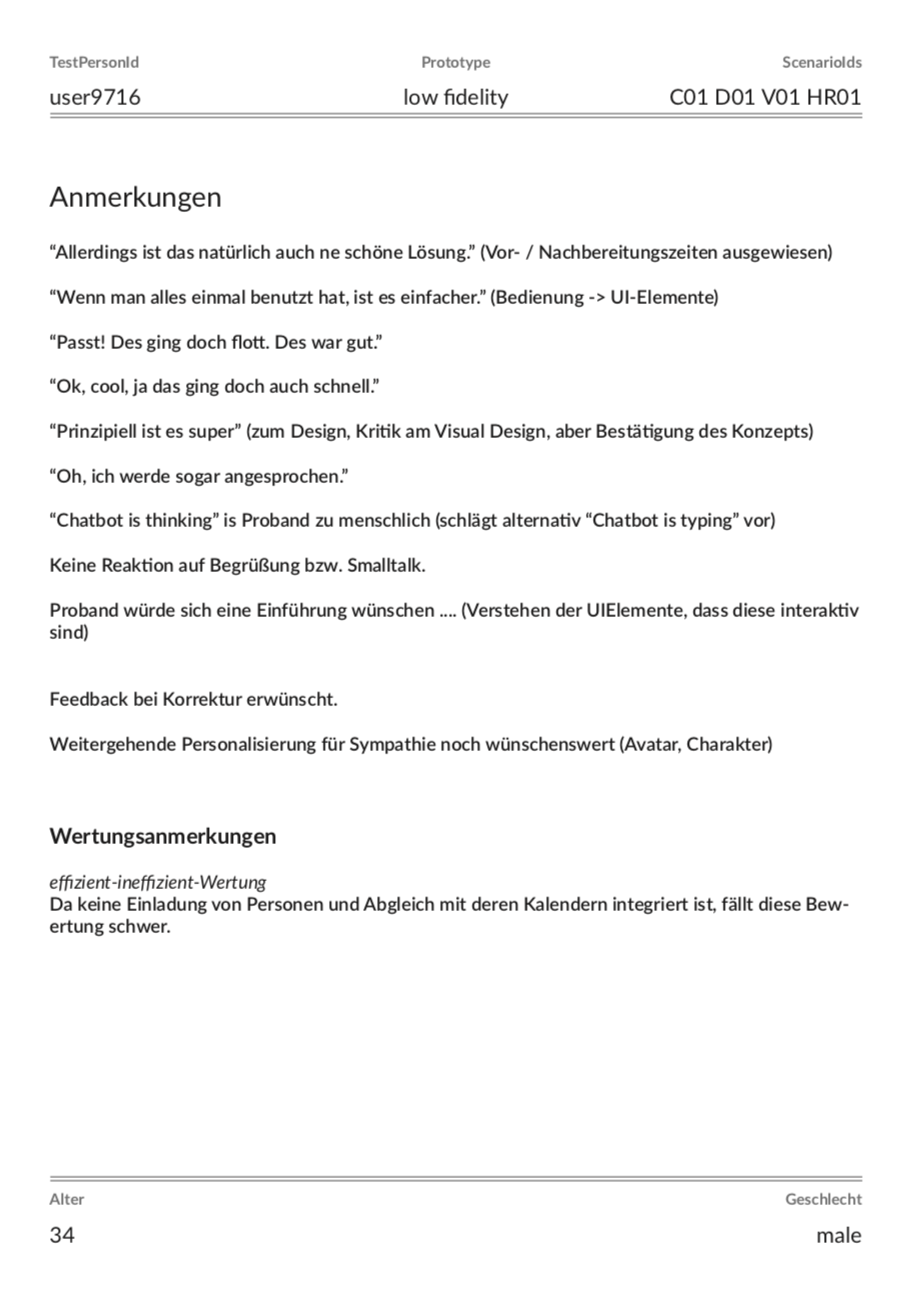
\includegraphics[width=0.9\textwidth]{bilder/anhang/UserTestAdorsys/user9716-back.png}}
    \caption{Notizen zum Fragebogen von user9716}
    \label{fig:feedback-user9716-back}
\end{figure}

%%%%%%%%%% CD Verzeichnisstruktur %%%%%%%%%%

\clearpage

\section{CD Verzeichnisstruktur}
\label{sec:cd-verzeichnisstruktur}
\begin{tabbing}
	mm \= mm \= mmmmmmmmmmmmmmmm \= \kill
    $\vdash$ \textbf{Latex-Files/} $\Rightarrow$ \textit{editierbare \LaTeX~Dateien}\\ %\llcorner
	\> \>  $\vdash$  \textbf{bilder/}   	\> $\Rightarrow$ \textit{Alle verwendeten Bilder}\\
	\> \>  $\vdash$  \textbf{hauptkapitel/}  \> $\Rightarrow$ \textit{Fünf Hauptkapitel}\\
	\> \>  $\vdash$  \textbf{literatur/}   \> $\Rightarrow$ \textit{Bibliotheksdatei und Zitierstil}\\
	\> \>  $\vdash$  \textbf{nebenkapitel/}   \> $\Rightarrow$ \textit{Deckblatt, Abstract, Anhang, ...}\\
	\> \> --config.tex\\
	\> \> --main.tex\\
	|\\
	$\vdash$ \textbf{Literatur/} \\ 
	\> \>  $\vdash$  \textbf{Android/} \\
	\> \>  $\vdash$  \textbf{CUI/} \\ 
	\> \>  $\vdash$  \textbf{Server-Technologien/} \\ 
	\> \>  $\vdash$  \textbf{Usability/} \\ 
	|\\
	$\vdash$ \textbf{Quelltexte/} $\Rightarrow$\\ %\llcorner
	\> \>  $\vdash$  \textbf{AndroidApp/}   	\> $\Rightarrow$ \textit{Android Applikation}\\
	\> \>  $\vdash$  \textbf{Dialogflow/}   	\> $\Rightarrow$ \textit{Dialogflow Agent}\\
	\> \>  $\vdash$  \textbf{PrototypingTool/}   	\> $\Rightarrow$ \textit{\ac{JSON}-Files der Szenarien}\\
	\> \>  $\vdash$  \textbf{Server/}   	\> $\Rightarrow$ \textit{Node.js Webservice}\\
    |\\
    $\vdash$ \textbf{Weiteres/} \\
    \> \>  $\vdash$  \textbf{AppVideos/}   	\> $\Rightarrow$ \textit{Beispielvideos zur Android Applikation}\\
	\> \>  $\vdash$  \textbf{Dokumente/}   	\> $\Rightarrow$ \textit{Exposee, Masterarbeit, Praesentation}\\
	|\\
\end{tabbing}